\chapter{Hardware}
\label{chap:hardware}
\lettrine[lines=3]{T}{his} chapter describes the hardware used to realize out
the project. Where the use of the Raspberry Pi single board computer designed to
have high performance both in education and science coupled with 8 mega-pixel
camera module CMOS sensor was an almost conditioned choice. Shows that
scientific and engineering--grade imagery can be produced with the Raspberry Pi
3 and its V2.1 camera module. It also presents a brief introduction to
thermography and its physical principles before introducing Lepton 2.5 thermal
camera module, made by the company FLIR which is currently one of the top
manufactures of thermal camera solutions. The Coral Dev Board is a single-board
computer that contains an Edge TPU coprocessor. It's ideal for prototyping new
projects that demand fast on-device inferencing for machine learning models. The
Coral Dev Board is ideal when you need to perform fast machine learning (ML)
inferencing in a small form factor.
%
\section{Raspberry Pi 3}
\label{sec:raspi3}
The Raspberry Pi is a high-performance single-board computer designed to
experiment and solve real-world problems. This small computer supports a camera
module that uses a Sony IMX219 8 mega-pixel CMOS sensor.
%
\subsection{Specification}
\label{ssec:raspispecification}
As of early 2016, over 8 million Raspberry Pi's had been sold, making it one of
the most popular single-board computers on the
market.\cite{upton2016raspberry}\\ The Raspberry Pi credit-card-sized computer
supports several accessories, including a camera module containing the Sony
IMX219 sensor. This computer and camera configuration is of particular interest
since it can provide raw-data format imagery that can be used for a multitude of
applications, including computer vision, biophotonics, medical testing, remote
sensing, astronomy, improved image quality, high dynamic range (HDR) imaging,
and security monitoring. The Raspberry Pi 3 is the third generation single board
Raspberry Pi computer and became available to consumers in February 2016. \\Some
of the more significant Raspberry Pi attributes, including interfaces, are
described in Table \ref{tab:rapberryattributes}. The Raspberry
Pi Foundation provides several operating systems for the  Raspberry Pi 3,
including Raspbian and a Debian-based Linux distribution, as  well as
third-party Ubuntu, Windows 10 IOT Core, RISC OS, and specialized  distributions
for download.\cite{10.1117/1.JEI.26.1.013014}
%
\begin{table}[htb]
\centering
	\caption{Raspberry Pi 3 computer attributes.}
	\label{tab:rapberryattributes}
	\begin{tabular}{l}
		\hline
		CPU 1.2 \si{\giga\hertz} 64-bit ARM Cortex-A53 \\
		1 GB of RAM LPDDR2 (900 \si{\mega\hertz}) \\
		Wireless N and Blue-tooth 4.1 communication\\
		Four USB ports\\
		HDMI interface\\
		Ethernet port\\
		MicroSD card slot\\
		40 GPIO pins\\
		Camera interface\\
		Composite video audio jack\\
		\hline
\end{tabular}
\end{table}
%
\section{Raspberry Pi, Camera Board V2}
\label{sec:raspicam}
The camera is based on the Sony IMX219 silicon CMOS back-lit sensor and produces
8 mega-pixel images that are $3280 \times 2464$ pixels in size. \\
The IMX219 sensor operates in the visible spectral range from 400 to 700 \si{\nano\meter}).\cite{raspberrycam2}
Sensor specifications are detailed in Table \ref{tab:raspicamspec}.
%
\begin{table}[!h]
	\centering
	\caption{Sony IMX219 sensor chip specifications.}
	\label{tab:raspicamspec}
	\begin{tabular}{l l}
		\hline
		\textbf{Sensor parameter}			& 	\textbf{Specification}\\
		\hline
		Image sensor type		&	Back-lit CMOS\\
		Image size				&	Diagonal 4.60 \si{\milli\meter} (type 1/4.0)\\
		Number of active pixels	&	3280 (H) $\times$ 2464 (V) $\sim$ 8.08 mega-pixels\\
		Chip size				&	5.095 \si{\milli\meter} (H) $\times$ 4.930 \si{\milli\meter}(V) (w/ Scribe)\\	
		Unit cell size (pixel) 	&	1.12 \si{\micro\meter} (H) $\times$ 1.12 \si{\micro\meter}(V)\\
		Substrate material		&	Silicon\\
		Bit depth				&	10-bit A/D converter on chip\\
		Data output				&	CSI2 serial data output (selection of 4 lane/ 2 lane)\\
		Communication			&	2-wire serial communication circuit on chip\\
		Max full-frame frame rate &	30 frames/s \\
		Pixel rate 				&	280 mega-pixel/s (all-pixels mode)\\
		Data rate				&	Max. 755 Mbps/lane (at 4 lane), 912 Mbps / lane(at 2 lane)\\
		\hline
	\end{tabular}
\end{table}
%
\subsection{Specification}
\label{ssec:raspcamspecification}
The V2 camera module operates at a fixed focal length (3.04 \si{\milli\meter})
and single $f$-number (F$2.0$) typically focused from the near-field to
infinity. Images can be captured at ISO settings between 100 and 800 in manually
set increments of 100
and camera exposure times between \SI{9}{\micro\second} and 6 \si{\second} using
a rolling shutter. Some of the more significant camera specifications are shown
in Table \ref{tab:raspicamspec2}. In addition to still photos, the Raspberry Pi
Sony IMX219 sensor supports a cropped 1080p format at 30 frames per second (fps)
and full-frame imaging video at up to 15 fps, but not in raw-data format. The
entire camera board is small 25 \si{\milli\meter} $\times$ 25 \si{\milli\meter}
$\times$ 9 \si{\milli\meter} and weighing about $3$ \si{\gram}. It connects
directly to the Raspberry Pi 3 through a 15 pin mobile industry processor
interface (MIPI) camera serial interface and is shown alongside a Raspberry Pi 3
in Figure \ref{fig:boardcam}.\cite{upton2016raspberry, raspberrycam}
%
\begin{table}[htb]
	\centering
	\caption{Raspberry Pi camera.}
	\label{tab:raspicamspec2}
	\begin{tabular}{l l}
		\hline
		\textbf{Camera parameter}			& 	\textbf{Specification}\\
		\hline
		Lens focal length 	& 	3.04 \si{\milli\meter}	\\
		$f$-number			&	2.0	\\
		Instantaneous field of view	&	0.368 \si{\milli\radian}\\
		Full-frame field of view & 59.17 \si{\degree}(H) $\times$ 58.3 \si{\degree} (V)\\
		\hline
	\end{tabular}
\end{table}
%

\begin{figure}[htb]
	\centering
    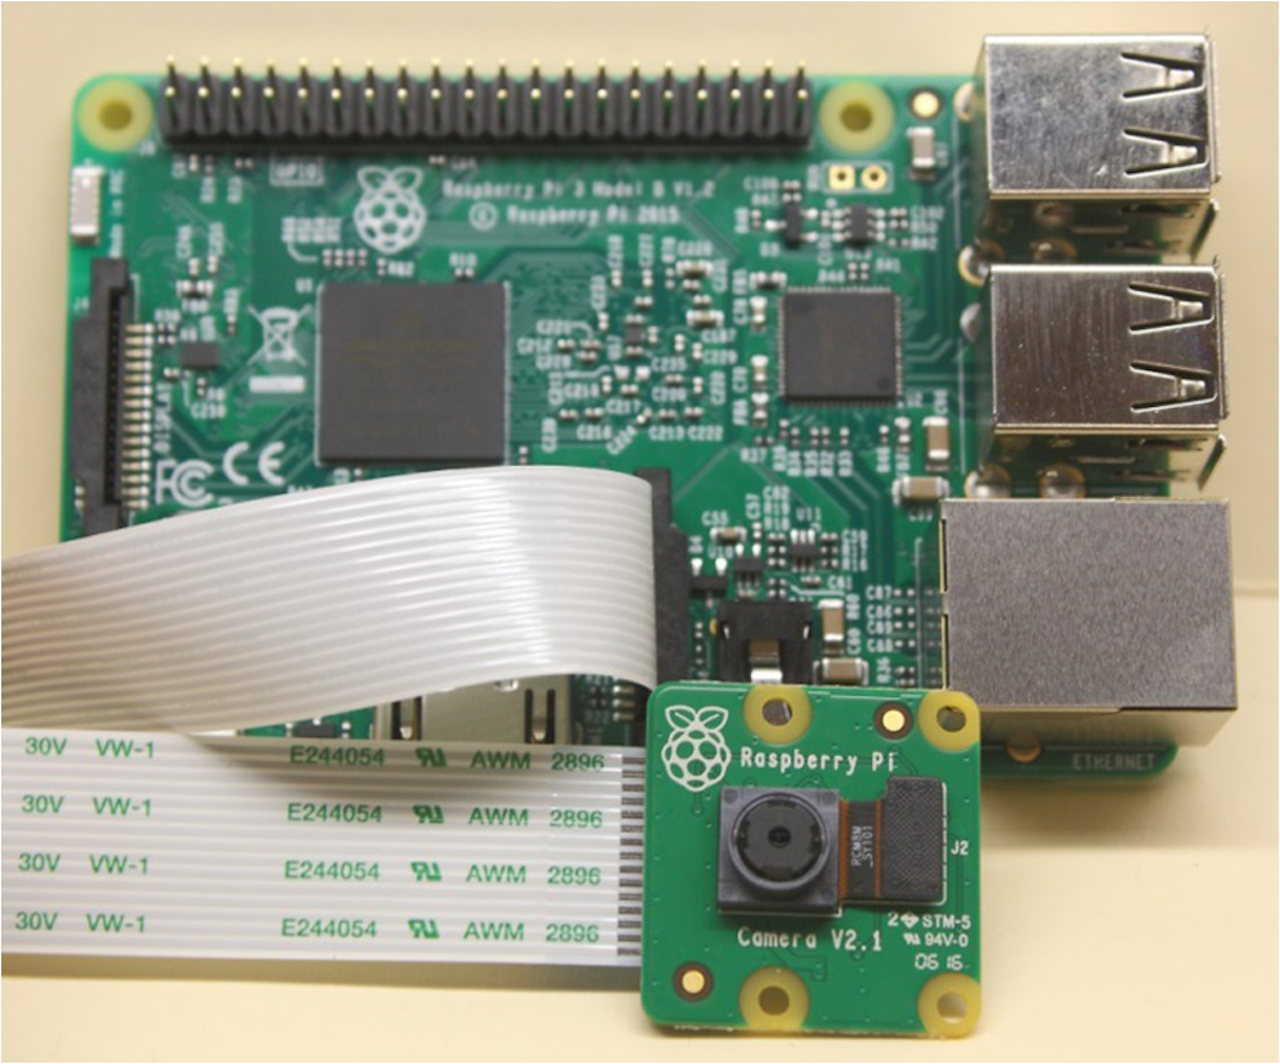
\includegraphics[width=0.80\textwidth]{JEI_26_1_013014_f001.png}
    \caption{Raspberry Pi 3 and camera module V2.1.}
    \label{fig:boardcam}
\end{figure}
\section{Thermal imaging theory}
\label{sec:theory}
The story of infra-red imaging started in 1800, when Herschel discovered 
infra-red radiation experimentally at long wavelengths just outside the visible 
spectrum of sun light.
The quantitative explanation of incandescent infra-red radiation in 1900 by Max 
Planck started a development, which today has resulted in modern infra-red 
technologies with infra-red camera systems These are also the result of 
scientific developments in semiconductor physics and micro-system 
technologies.\cite{10.1117/12.2266142}
Since its birth, it is possible to recognize three generations of infra-red 
cameras\cite{thermalimage}: the first generation cameras were characterized by 
a single element detector, combined with two scanning mirrors to create 
infra-red images. 
Their main disadvantage was that they suffered from saturation problems. 
Saturation indicates the limit of the highest irradiation that can be measured 
by a detector. For digital sensors, since incident photoelectrons are converted 
in charges, each detector can store a maximum amount of charges known as the 
full well capacity.\cite{10.1117/12.2266142}
The second generation cameras were characterized by an increase in the number 
of detectors, positioned in a large linear array or in two small 2-D array.
The third generation cameras, i.e., the ones currently used, are characterized 
by large focal plane array (FPA) detectors, thus increasing the reliability 
and sensitivity of such infra-red systems.\cite{rogalski2000infrared} 
%
\subsection{Electromagnetic radiation}
\label{ssec:electromagnetic-radiation}
Electromagnetic radiation is all around (and within, and throughout) us and is
comprised of everything from gamma radiation on the high frequency end to radio
waves on the low frequency end. So the Figure (\ref{fig:spectrum}) give an
overview of EM waves, ordered according to their wave-length or frequency. 
This spectrum consists of a great variety of different waves. All of them can
be observed in nature, and many have technical applications. Starting from the
left of the figure, for example, $\gamma$-rays have the highest frequencies,
that is, the shortest wavelengths.\cite{vollmer2017infrared} \hfill \break
%
%
\begin{figure}[htb]
	\centering
	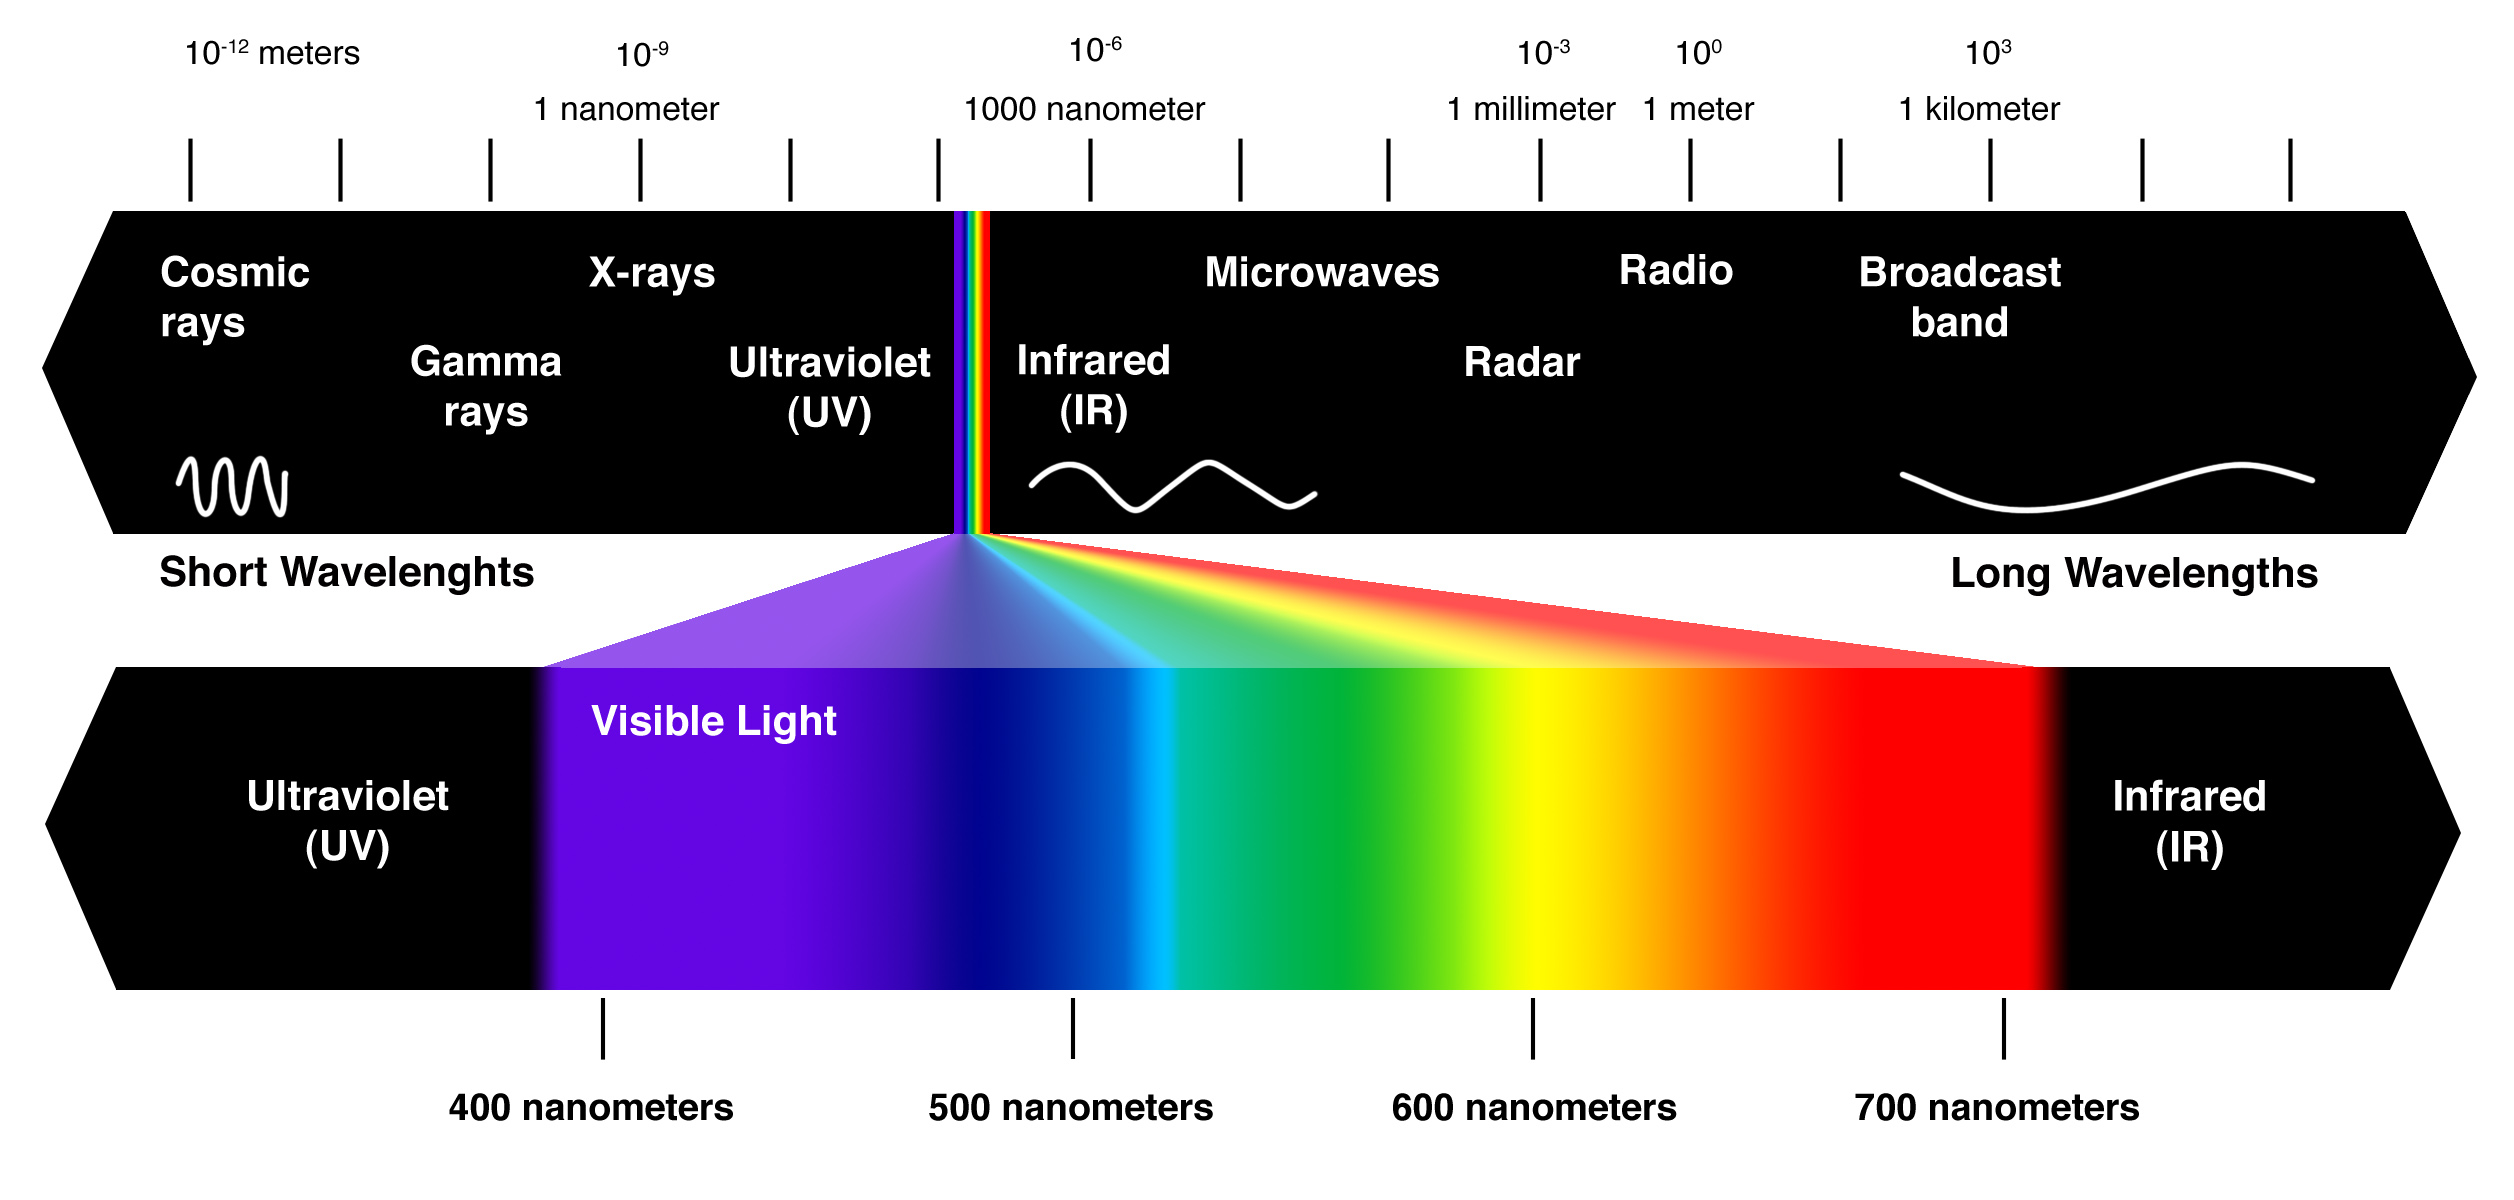
\includegraphics[width=0.65\textwidth]{Visible-spectrum.jpeg}
	\captionsource{Composition of the spectrum of electromagnetic waves.}{
	\href{https://socratic.org/questions/what-is-the-wavelength-of-a-photon-of-blue-light-whose-frequency-is-6-3-10-14-s-}{https://socratic.org}}
	\label{fig:spectrum}
\end{figure}
%
\newline
The visible light, defined by the sensitive range of the light receptors in our
eyes, only covers a very small range within this spectrum, with wavelengths from
$380$ to $780$ \si{\nano\meter}. The adjacent spectral region with wavelengths
from $780$ \si{\nano\meter} up to $1$ \si{\milli\meter} is usually called infra-red. 
This range is followed by microwaves, RADAR, and all EM waves that are used for
radio, TV, and so on.
While most imaging sensors detect radiation in the visible spectrum (wavelengths
from $380$ to $700 \,\si{\nano\meter}$), long wave infra-red sensors detect
radiation the infra-red spectrum, and it accounts for most of the thermal
radiation emitted by objects near room temperature. Then for IR imaging, only a
small range of the IR spectrum is used. It is shown in an expanded view in
Figure (\ref{fig:spectrum-ir}). Typically, three spectral ranges are defined for thermography: 
the long-wave (LW) region from around $8$ to $14$ \si{\micro\meter}, the
mid-wave (MW) region from around $3$ to $5$ \si{\micro\meter}, and the 
short-wave (SW) region from $0.9$ to $1.7$ \si{\micro\meter}.
%
%
\begin{figure}[!h]
	\centering
	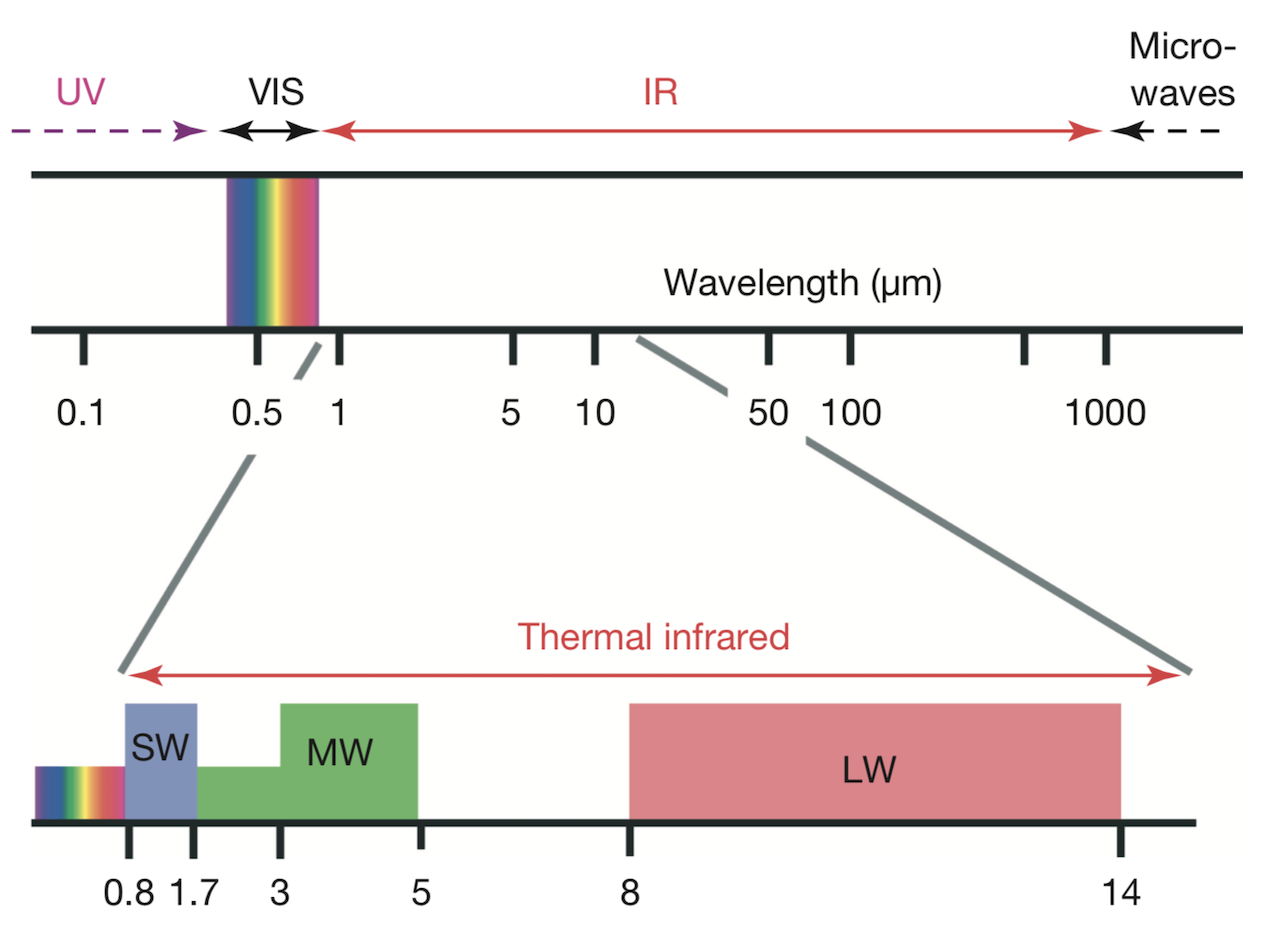
\includegraphics[width=0.65\textwidth]{spectrum-ir.png}
	\captionsource{Infrared (IR) and adjacent spectral regions and expanded view of so-called thermal IR. This is the region where IR imaging systems for short-wave (SW), mid-wave (MW), and long- wave (LW) cameras exist. Special systems have extended ranges.
}{\cite{vollmer2017infrared}}
	\label{fig:spectrum-ir}
\end{figure}
% 
The origin of naturally occurring EM radiation is manifold. 
The most important phenom for thermography is the thermal radiation. 
In brief, the thermal radiation implies that every body or object at a
temperature T $>0 \,$ \si{\kelvin} $\,(-273.15 \,$\si{\celsius}$)$ emits EM
radiation. 
The amount of radiation and its distribution as a function of wavelength depend
on temperature and material properties. \cite{vollmer2017infrared} 
For temperatures in the range of natural and technological processes, this 
radiation is in the thermal IR spectral region. 
This is known as the infra-red spectrum, and it accounts for most of the
thermal radiation emitted by objects near room temperature.
%
\subsection{Modern detectors}
\label{ssec:modern-detect}
The main difference between a thermal imaging and normal image capturing is the
sensor used. One type of the sensor used in thermal cameras is called a
microbolometer. Essentially its functionality is similar to the CMOS or CCD
sensor, just in different wavelengths. Unlike many other thermal sensor the
microbolometer doesn't need an active cooling system to function a long period
of times. Modern uncooled detectors use sensors whose working mechanism is based
on a change of resistance, voltage or current when heated by IR radiation.
Uncooled detectors are mostly composed by pyroelectric and ferroelectric
materials or based on microbolometer technology. The thermal signal depends upon
the radiant power but not upon its spectral content, i.e., it is wavelength
independent.\cite{10.1117/12.2266142,rogalski2000infrared}

\section{Thermal Camera module Lepton 2.5}
\label{sec:thermalcamera}
The thermal camera module we use in this project, we will go through its
specification, modes of capture and communication protocol for both video frame
transfer and camera control. Information about the camera are extracted from
official documentation.

% TODO CHECK DOCUMENTATION AND LINK IN REFERENCE-BIBLIOGRAPHY

% TODO INSERT IMAGE FLIR LEPTON

\subsection{Specification}
\label{ssec:specificationthermalcam}
Lepton is an infra-red camera system that integrates a fixed-focus lens assembly,
an $80 \times 60$ long-wave infra-red (LWIR) micro-bolometer sensor array, and
signal-processing electronics. Easy to integrate and operate, Lepton is intended
for mobile devices as well as any other application requiring very small
footprint, very low power, and instant-on operation. Lepton can be operated in
its default mode or configured into other modes through a command and control
interface (CCI). The effective frame rate of the camera is only 8.6 \si{\hertz},
however for our needs this is not a problem. The camera only requires low
voltage supply and has small power consumption of around 140 \si{\milli\watt}.
%
\begin{table}[htb]
    \centering
    \caption{Key Specifications}
    \label{tab:thcamspecifications}
    \begin{tabular}{l c c}
        \hline
                                                            &   FLIR Lepton 2.5 	&          	\\
        \hline
        \rowcolor{aliceblue!85} Resolution (h x w)	       	&   80 $\times$ 60  	&	pixels	\\
        Spectral Range	                                    	&   8  to 14        	&	\si{\micro\meter}	\\
        \rowcolor{aliceblue!85} Horizontal Field of View		&   51              	&   \si{\degree}			\\
        Thermal Sensitivity	                                	&   < 50            	&   \si{\milli\kelvin}	\\
        \rowcolor{aliceblue!85} Frame Rate	                	&   < 9             	&   \si{\hertz} 			\\
        Control Interface	                                	&   I$^{2}$C        	&               			\\
        \rowcolor{aliceblue!85} Video Interface	            	&   SPI             	&               			\\
        Promised Time to Image	                            	&   < 0.5           	&   \si{\second}    		\\
        \rowcolor{aliceblue!85} Integral Shutter		    		&   yes             	&   			\\
        Radiometry	                                        	&   14-bit pixel value  	&       \\
        \rowcolor{aliceblue!85} Operating Power             	&	$\sim$150       	&   \si{\milli\watt} 	\\
        \hline
\end{tabular}
\end{table}
%
See table \ref{tab:thcamspecifications} for more specifications.\\For better
manipulation with the camera module we use a breakout board (figure 3.1) with a
housing for the Lepton camera module. The breakout board provides better
physical accessibility, improves heat dissipation and increases input voltage
supply range to 3--5 \si{\volt}, as it has its own regulated power supply. This
power supply provides the camera module with three necessary voltages: 1.2, 2.8
and 2.5--3.1 \si{\volt}. The breakout board also supplies the camera with master
clock signal. [14] \\
The camera uses two interfaces for communication:
\begin{itemize}
    \item SPI for transferring video frames from the camera to a SPI master
device.
    \item I$^{2}$C for receiving control commands from the I$^{2}$C master
device.
\end{itemize}
Even though the name of the project include the keyword low-cost, we need to
think of this statement with respect to the thermal camera market. The Lepton 3
thermal camera module can be considered low-cost when compared to other thermal
camera devices available as it costs around $250$ (2018) 4. This could however
be considerably more when compared to other nonthermal solutions, however way
more than if we would utilize a simple infra-red counting sensors for example.
%
\begin{figure}[htb]
    \centering
    \resizebox{0.8\textwidth}{!}{
\begin{tikzpicture}
    \draw[help lines] (0,0) grid (20, 20);
%     \draw (0,0) rectangle (10,20);
% \draw[fill=cyan!50] (1,1) rectangle (7,3)   node {Camera Supply Inputs};
% \draw[fill=cyan!50] (1,3) rectangle (7,6)   node {Camera Shut Down};
% \draw[fill=cyan] (1,6) rectangle (7,11) node {Camera Reset};
% \draw[fill=cyan!50] (1,11) rectangle (7,13) node {Camera Clock Gneration};
% \draw[fill=cyan!50] (1,13) rectangle (7,15) node {Camera };
% \draw[fill=cyan!50] (1,15) rectangle (7,17) node {Camera };
% \draw[fill=cyan!50] (1,17) rectangle (7,19) node {Camera };
% \draw[fill=cyan!50] (1,1) rectangle (,);
% \draw[fill=cyan!50] (1,1) rectangle (,);
% \draw[fill=cyan!50] (1,1) rectangle (,);
% \draw[fill=cyan!50] (1,1) rectangle (,);
% \draw[fill=cyan!50] (1,1) rectangle (,);
% \draw[fill=cyan!50] (1,1) rectangle (,);
% \draw[fill=cyan!50] (1,1) rectangle (,);
% \draw[fill=cyan!50] (1,1) rectangle (,);
% \draw[fill=cyan!50] (1,1) rectangle (,);
% \draw[fill=cyan!50] (1,1) rectangle (,);
% \draw[fill=cyan!50] (1,1) rectangle (,);
% \draw[fill=cyan!50] (1,1) rectangle (,);
% \draw[fill=cyan!50] (1,1) rectangle (,);
% \draw[fill=cyan!50] (1,1) rectangle (,);
% \draw[fill=cyan!50] (1,1) rectangle (,);








\end{tikzpicture}
}
    \caption{my figure drawn in tikz}\label{fig:myfigure}
\end{figure}
%
\subsection{System Architecture}
\label{ssec:leptonarchitecture}
The lens assembly focuses infrared radiation from the scene onto an $80 \times 60$ array
of thermal detectors with 17-micron pitch. Each detector element is a
vanadium-oxide (VOx) microbolometer whose temperature fluctuates in response to
incident flux. The change in temperature causes a proportional change in each
microbolometer’s resistance. VOx provides a high temperature coefficient of
resistance (TCR) and low 1/f noise, resulting in excellent thermal sensitivity
and stable uniformity. The microbolometer array is grown monolithically on top
of a readout integrated circuit (ROIC) to comprise the complete focal plane
array (FPA). Once per frame, the ROIC senses the resistance of each detector by
applying a bias voltage and integrating the resulting current for a finite
period of time called the integration period. The serial stream from the FPA is
received by a system on a chip (SoC) device, which provides signal processing
and output formatting.
%
\begin{figure}[htb]
    \centering
    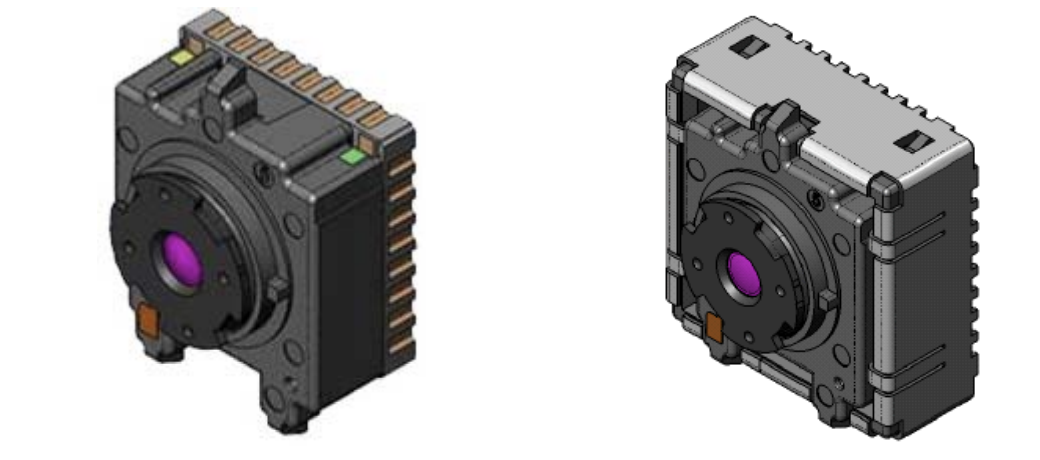
\includegraphics[width=0.80\textwidth]{leptoncamera.png}
    \caption{Lepton Camera (with and without socket)}
    \label{fig:camerarender}
\end{figure}
%
\subsection{video pipeline}
\label{ssec:pipeline}
The video pipeline includes non-uniformity correction (NUC), defect replacement,
spatial and temporal filtering, automatic gain correction (AGC), and
colourization.
%
%insert image video stream
%
% nuc
\paragraph{The non-uniformity correction (NUC)} block applies correction
terms to ensure that the camera produces a uniform output for each pixel when
imaging a uniform thermal scene. Factory-calibrated terms are applied to
compensate for temperature effects, pixel response variations, and
lens-illumination roll-off. To compensate for temporal drift, the NUC block also
applies an offset term that can be periodically updated at runtime via a process
called flat-field correction (FFC). The FFC process is further described in FFC
States, (\ref{ssec:FFCstates}).
%
%7.2 Defect Replacement
\paragraph{The defect-replacement} block substitutes for any pixels identified
as defective during factory calibration or during runtime. The replacement
algorithm assesses the values of neighboring pixels and calculates an optimum
replacement value. The typical number of defective pixels is $\leq 1$.
%
\paragraph{Temporal Filtering} the image pipeline includes a number of
sophisticated image filters designed to enhance signal-to-noise ratio (SNR) by
eliminating temporal noise and residual non-uniformity. The filtering suite
includes a scene-based non-uniformity correction (SBNUC) algorithm which relies
on motion within the scene to isolate fixed pattern noise (FPN) from image
content.
%
\paragraph{The AGC algorithm} for converting the full-resolution (14-bit)
thermal image into a contrast-enhanced image suitable for display is a
histogram-based non-linear mapping function. See (\ref{ssec:AGCModes}).
%
\paragraph{The colorize block} takes the contrast-enhanced thermal image as
input and generates a 24-bit RGB color output.
%
\subsection{Power States}
\label{ssec:powerstate}
Lepton currently provides five power states. As depicted in the state diagram
shown in Figure 6, most of the transitions among the power states are the result
of explicit action from the host. The automatic transition to and from the
overtemp state is an exception. In the figure, transitions that require specific
host-side action are shown in bold. Automatic transitions are not bolded.
%
\begin{itemize}
    \item Off: When no voltage is applied, Lepton is in the off
state. In the off state, no camera functions are available.
    \item Uninitialized:
In the uninitialized state, all voltage forms are applied, but Lepton has not
yet been booted and is in an indeterminate state. It is not recommended to leave
Lepton in this state as power is not optimized; it should instead be booted to
the on-state (and then transitioned back to standby if imaging is not required).
    \item On: In the on state, all functions and interfaces are fully available.
    \item Standby: In the standby state, all voltage forms are applied, but power
consumption is approximately 4 \si{\milli\watt}. In the standby state, no
functions are available, but it is possible to transition to the on state via
the start-up sequence defined in Figure 7 on page 16. The shutdown sequence
shown in Figure 7 on page 16 is the recommended transition back to the standby
state. It is also possible to transition between standby and on states via
software commands, as further defined in the software IDD.
    \item Overtemp: The
overtemp state is automatically entered when the Lepton senses that its
temperature has exceeded approximately $80$ \si{\celsius}. Upon entering the
overtemp state, Lepton enables a ``\emph{shutdown imminent}" status bit in the
telemetry line and starts a $10$ \si{\second} counter. If the temperature of the
Lepton falls below $80$ \si{\celsius} before the counter times out, the
``\emph{shutdown imminent}" bit is cleared and the system transitions back to
the on state. If the counter does time out, Lepton automatically transitions to
the standby state.
\end{itemize}
%
\subsection{FFC States}
\label{ssec:FFCstates}
Lepton is factory calibrated to produce an output image that is highly uniform,
such as shown in Figure \ref{subfig:Highly uniform image}, when viewing a
uniform-temperature scene. However, drift effects over long periods of time
degrade uniformity, resulting in imagery which appears more grainy (Figure
\ref{subfig:Grainy image}) and/or blotchy (Figure \ref{subfig:Blotchy image}).
Operation over a wide temperature range (for example, powering on at $-10$
\si{\celsius} and heating to $65$ \si{\celsius}) will also have a detrimental
effect on image quality. For scenarios in which there is ample scene movement,
such as most handheld applications, Lepton is capable of automatically
compensating for drift effects using an internal algorithm called scene-based
non-uniformity correction (scene-based NUC or SBNUC). However, for use cases in
which the scene is essentially stationary, such as fixed-mount applications,
scene-based NUC is less effective. In those applications, it is recommended to
periodically perform a flat-field correction (FFC). FFC is a process whereby the
NUC terms applied by the camera's signal processing engine are automatically
recalibrated to produce the most optimal image quality. The sensor is briefly
exposed to a uniform thermal scene, and the camera updates the NUC terms to
ensure uniform output. The entire FFC process takes less than a second.
%
\begin{figure}[htb]
    \centering
    \subfloat[][\emph{Highly uniform image}.\label{subfig:Highly uniform image}]
        {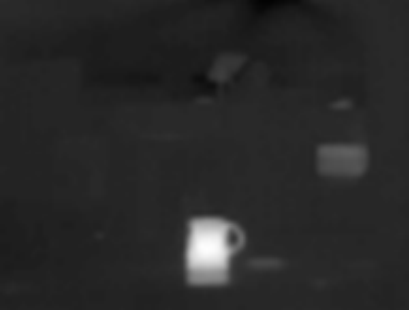
\includegraphics[width=.30\textwidth]{linearAGCa}} \quad
    \subfloat[][\emph{Grainy image
    (high-spatial frequency noise)}.\label{subfig:Grainy image}]
        {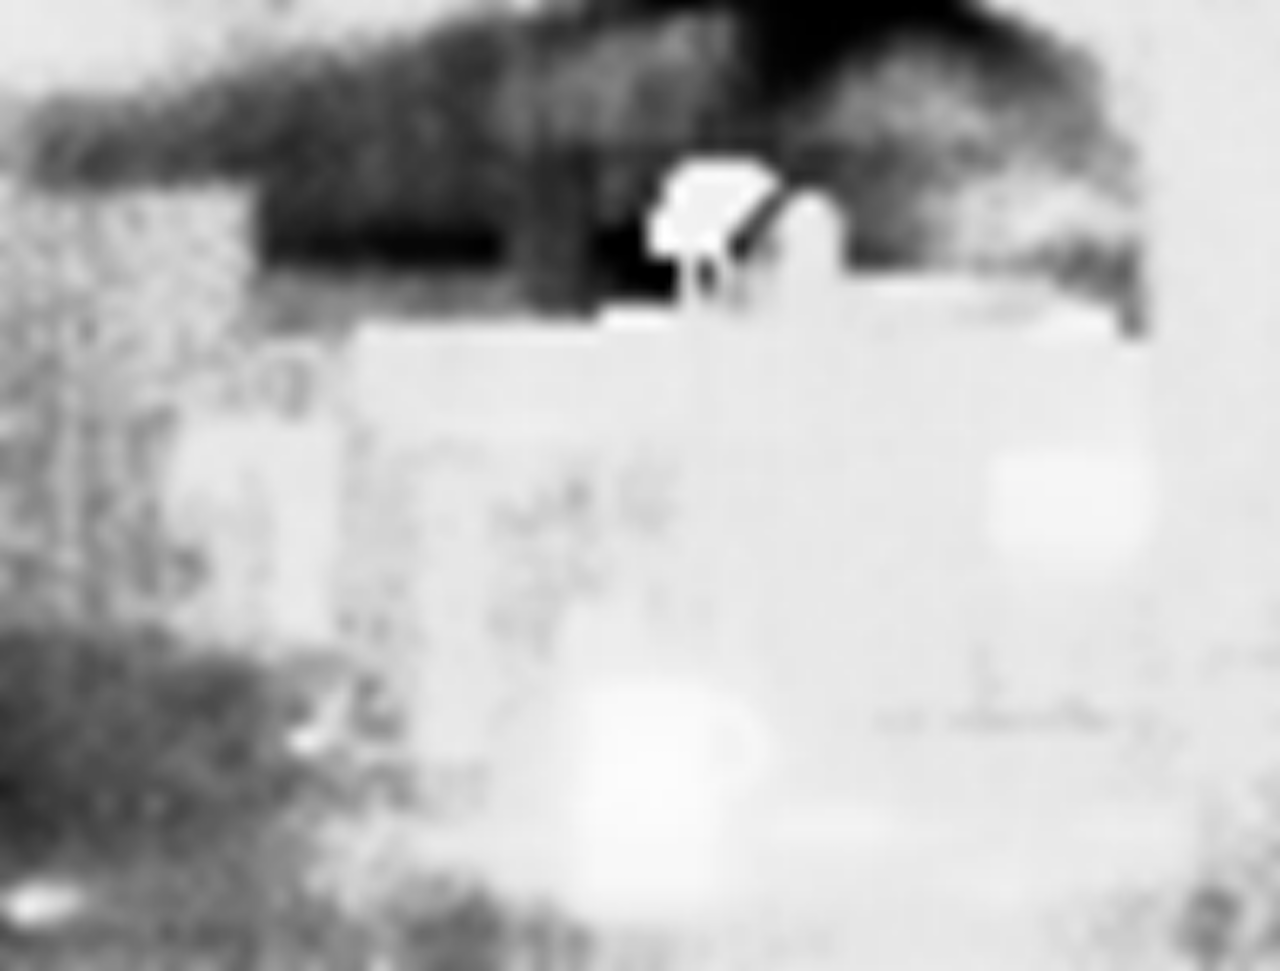
\includegraphics[width=.30\textwidth]{linearAGCb.png}} \quad
    \subfloat[][\emph{ Blotchy image
    (low-spatial frequency noise)}.\label{subfig:Blotchy image}]
        {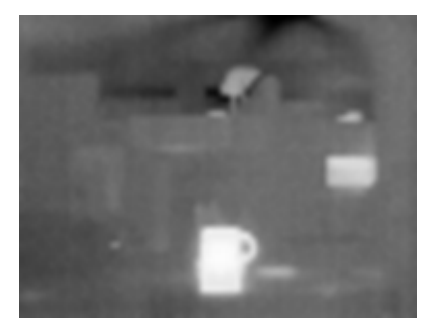
\includegraphics[width=.30\textwidth]{linearAGCc.png}}
    \caption{Examples of Good Uniformity, Graininess, and Blotchiness}
    \label{fig:exampleffc}
\end{figure}
%
\\The current FFC state is provided through the telemetry line. There are three
FFC states, as illustrated in Figure \ref{fig:FFC States}:
\begin{enumerate}
    \item FFC not commanded (default): In this state, Lepton applies by default a
set of factory-generated FFC terms.
    \item FFC in progress: Lepton enters this
state when FFC is commanded. The default FFC duration is nominally $23$ frames.
    \item FFC complete: Lepton automatically enters this state whenever FFC is
completed. Lepton also provides an ``FFC desired" flag in the telemetry line.
The ``FFC desired" flag is asserted at start-up, when a specified period
(default = 3 minutes) has elapsed since the last FFC, or when the sensor
temperature has changed by a specified value (default = 3 \si{\celsius}) since
the last FFC. The ``FFC desired" flag is intended to indicate to the host to
command an FFC at the next possible opportunity.
\end{enumerate}
%
\begin{figure}[htb]
    \centering
    \resizebox{0.35\textwidth}{!}{\begin{tikzpicture}
    \node (start) at (1,12) {Lepton powered on};
    \node [ellipse, fill=babyblueeyes, align=center] (notcommand) at (1,10) {FFC Not \\ Commanded};
    \node [ellipse, fill=babyblueeyes] (progress) at (1,8) {FFC In Progress};
    \node [ellipse, fill=babyblueeyes] (complete) at (1,6) {FFC Complete};
    \draw [-latex] (start) to (notcommand);
    % connections
    \path[-latex] (notcommand)  edge [bend right=50]    node[left] {\tiny{FFC Commanded}} (progress);
    \path[-latex] (progress)    edge [bend left=50]     node[right] {\tiny{FFC Complete}} (complete);
    \path[-latex] (complete)    edge [bend left=50]     node[left] {\tiny{FFC Commanded}} (progress);
\end{tikzpicture}
}
    \caption{FFC States.}
    \label{fig:FFC States}
\end{figure}
%
\subsection{AGC Modes}
\label{ssec:AGCModes}
There are two AGC modes:
\begin{itemize}
    \item AGC disabled (default)
    \item AGC enabled
\end{itemize}
AGC is a process whereby the large dynamic range of the infrared sensor is
collapsed to a range more appropriate for a display system. For Lepton, this is
a 14-bit to 8-bit conversion. In its most simplistic form, AGC can be a linear
mapping from 14-bit to 8-bit; however, a simple linear AGC is generally
incapable of providing pleasing imagery in all imaging conditions. For example,
when a scene includes both cold and hot regions (for example, a hot object in
front of a cold background as illustrated in \ref{fig:comparisionlinearAGC},
linear AGC can produce an output image in which most pixels are mapped to either
full black or full white with very little use of the gray shades (8-bit values)
in between. Because of this limitation of linear AGC, a more sophisticated
algorithm is preferred. Similar to most AGC algorithms that optimize the use of
gray shades, Lepton's is histogram-based. Essentially a histogram counts the
number of pixels in each frame that have a given 14-bit value. Figure
\ref{fig:histogram} the concept for a 3x3 pixel area.\linebreak
%
\begin{figure}[!h]
    \centering
    \resizebox{0.80\textwidth}{!}{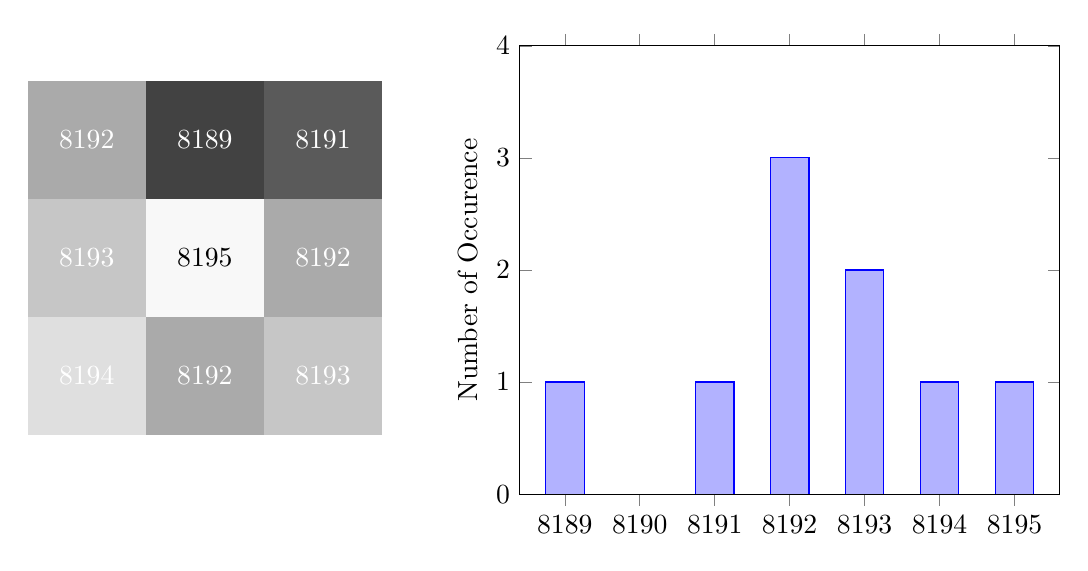
\begin{tikzpicture}
    \begin{scope}[xshift=-35mm]
        % upper row
        \node [rectangle, minimum size=15mm, fill={rgb,255:red,170; green,170; blue,170}](8192) at (1.5,4.5)   {\textcolor{white}{$8192$}};
        \node [rectangle, minimum size=15mm, fill={rgb,255:red,66; green,66; blue,66}](8189) at (3,4.5)     {\textcolor{white}{$8189$}};
        \node [rectangle, minimum size=15mm, fill={rgb,255:red,90; green,90; blue,90}](8191) at (4.5,4.5)   {\textcolor{white}{$8191$}};
        % mid row
        \node [rectangle, minimum size=15mm, fill={rgb,255:red,198; green,198; blue,198}](8193) at (1.5,3)     {\textcolor{white}{$8193$}};
        \node [rectangle, minimum size=15mm, fill={rgb,255:red,248; green,248; blue,248}](8195) at (3,3)       {\textcolor{black}{$8195$}};
        \node [rectangle, minimum size=15mm, fill={rgb,255:red,170; green,170; blue,170}](8192) at (4.5,3)     {\textcolor{white}{$8192$}};
        % lower row
        \node [rectangle, minimum size=15mm, fill={rgb,255:red,223; green,223; blue,223}](8194) at (1.5,1.5)   {\textcolor{white}{$8194$}};
        \node [rectangle, minimum size=15mm, fill={rgb,255:red,170; green,170; blue,170}](8192) at (3,1.5)     {\textcolor{white}{$8192$}};
        \node [rectangle, minimum size=15mm, fill={rgb,255:red,198; green,198; blue,198}](8193) at (4.5,1.5)   {\textcolor{white}{$8193$}};
    \end{scope}
    \begin{scope}[xshift=35mm]
        \begin{axis}[
            x tick label style={/pgf/number format/1000 sep=},
            ybar, bar width=14pt,
            ymin=0, ymax=4,
            ylabel = Number of Occurence,
            area style
        ]
    \addplot coordinates { (8189, 1) (8190, 0) (8191, 1) (8192, 3) (8193, 2) (8194, 1) (8195, 1) };
    \end{axis}
\end{scope}
\end{tikzpicture}
}
    \caption{Illustration of a Histogram for a $3 \times 3$ Pixel Area.}
    \label{fig:histogram}
\end{figure}
%
Classic histogram equalization uses the cumulative histogram as a
mapping function between 14-bit and 8-bit. The intent is to devote the most gray
shades to those portions of the input range occupied by the most pixels. For
example, an image consisting of $60 \%$ sky devotes $60 \%$ of the available
gray shades to the sky, leaving only $40 \%$ for the remainder of the image. By
comparison, linear AGC ``wastes" gray shades when there are gaps in the
histogram, whereas classic histogram equalization allocates no gray shades to
the gaps. This behavior is in principle an efficient use of the available gray
shades, but there are a few drawbacks:
\begin{itemize}
    \item The resulting contrast between an object and a much colder (or hotter)
background can be rendered poor by the fact the algorithm ``collapses" the
separation between such that the object is only one step gray shade above the
background. This phenomenon is illustrated in \ref{fig:comparisionlinearAGC}.
    \item Too much emphasis can be placed on background clutter, particularly
when a mostly isothermal background comprises a large fraction of the total
image area. This is also illustrated in \ref{fig:comparisionlinearAGC}. The
Lepton AGC algorithm is a modified version of classic histogram equalization
that mitigates these shortcomings. One such modification is a parameter called
``clip limit high". It clips the maximum population of any single bin, limiting
the influence of heavily populated bins on the mapping function. Another
parameter utilized by the Lepton algorithm is called ``clip limit low". It adds
a constant value to every non-zero bin in the histogram, resulting in additional
contrast between portions of the histogram separated by gaps. Figure
\ref{fig:comparisionlinearAGC} is an example showing the benefit of the Lepton
clip parameters.
%
\end{itemize}
\begin{figure}[!h]
    \centering
    \subfloat[][\emph{Linear AGC}.\label{subfig:linearagc}]
        {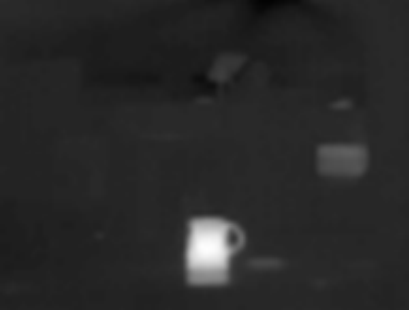
\includegraphics[width=.30\textwidth]{linearAGCa}} \quad
    \subfloat[][\emph{Classic Histogram Equalization}.\label{subfig:histrogram}]
        {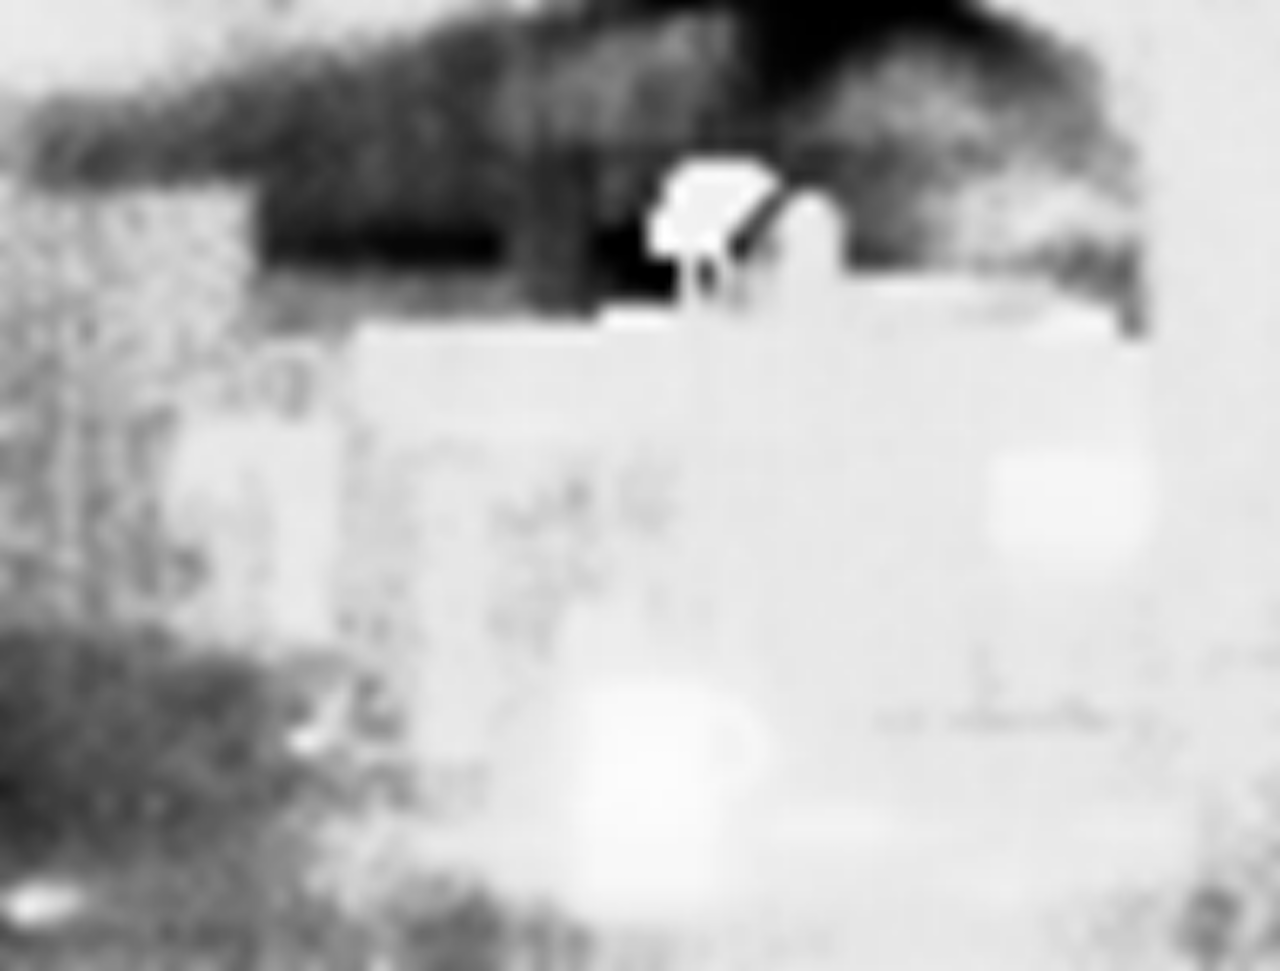
\includegraphics[width=.30\textwidth]{linearAGCb.png}} \quad
    \subfloat[][\emph{Lepton's Variant of HistogramEqualization}.\label{subfig:varianhistograms}]
        {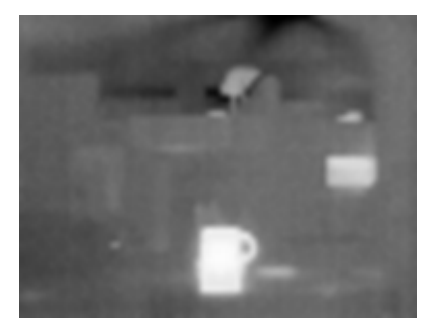
\includegraphics[width=.30\textwidth]{linearAGCc.png}}
    \caption{Comparison of Linear AGC and Classic/Lepton Variant of Histogram Equalization}
    \label{fig:comparisionlinearAGC}
\end{figure}
%
A high value of clip limit high results in a mapping more like classic histogram
equalization, whereas a low value results in mapping more like linear AGC. For
clip limit low, the opposite is true: a high value results in a mapping more
like linear AGC, whereas a low value results in a mapping more like classic
histogram equalization. The default values of both parameters produce a good
compromise between the two; however, because optimum AGC is highly subjective
and often application dependent, customers are encouraged to experiment to find
settings most appropriate for the target application. By default, the histogram
used to generate Lepton's 14-bit to 8-bit mapping function is collected from the
full array. In some applications, it is desirable to have the AGC algorithm
ignore a portion of the scene when collecting the histogram. For example, in
some applications it may be beneficial to optimize the display to a region of
interest (ROI) in the central portion of the image. When the AGC ROI is set to a
subset of the full image, any scene content located outside of the ROI is not
included in the histogram and therefore does not affect the mapping function
(note: this does not mean the portion outside of the ROI is not displayed or
that AGC is not applied there, only that those portions outside the AGC ROI do
not influence the mapping function).
%
%
\section{Interface}
\label{sec:lepton-interface}
The Raspberry Pi seen in section (\ref{sec:raspi3}) has bi-directional I/O pins, which you can use to drive LEDs, spin motors, or read button presses.
The board offers its GPIO over a standard male header on the board. Over the years the header has expanded from 26 pins to 40 pins while maintaining the original pinout.
There are at least two, different numbering schemes you may encounter when referencing pin numbers:
\begin{enumerate}
\item Broadcom chip-specific pin numbers 
\item \texttt{P1} physical pin numbers.
\end{enumerate} 
Here's a figure \ref{fig:gpio} showing all 26 pins on the \texttt{P1} header, including any special function they may have, and their dual numbers.
%
%
\begin{figure}[htb]
	\centering
	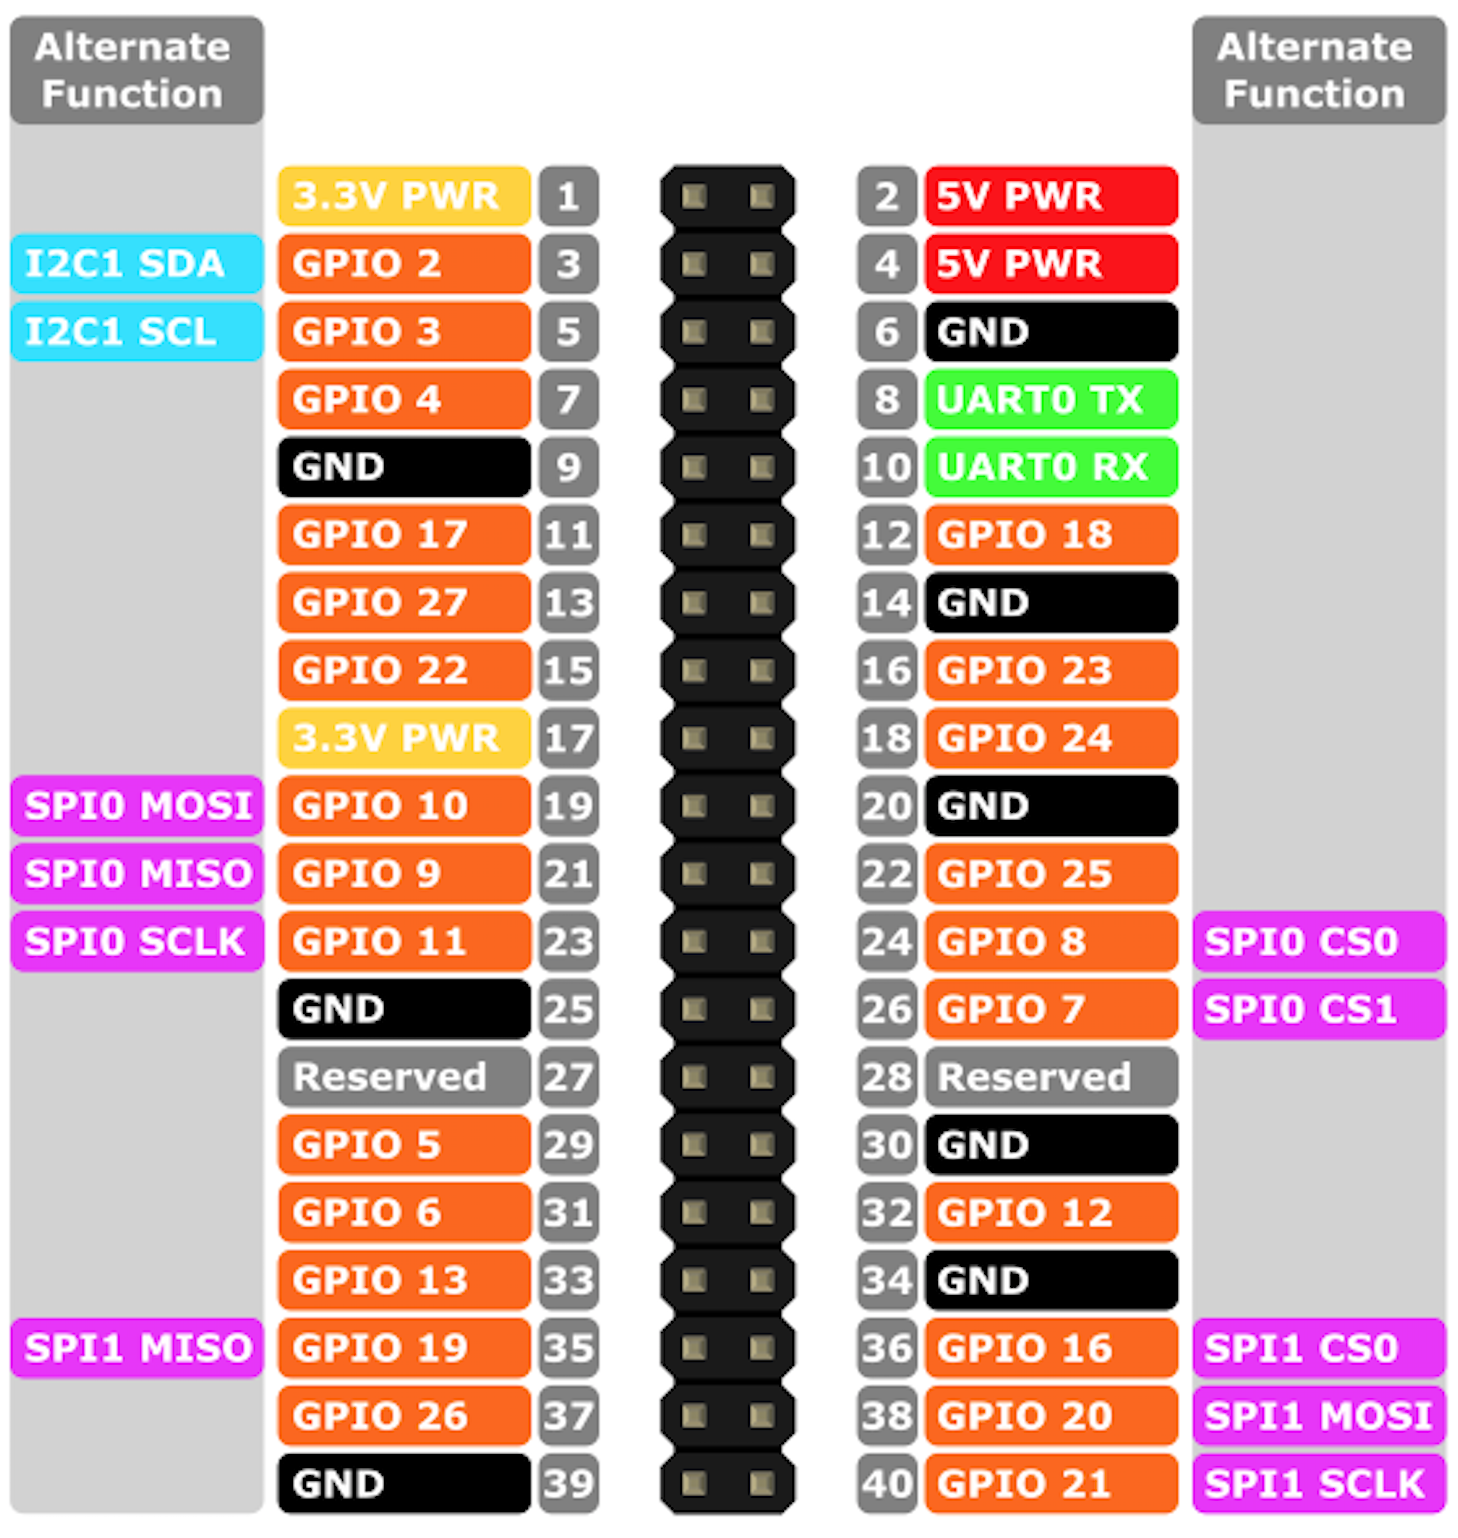
\includegraphics[width=0.45\textwidth]{gpio.png}
	\captionsource{Raspberry Pi 3 Pin Mappings.}{\href{https://docs.microsoft.com/es-es/windows/iot-core/learn-about-hardware/pinmappings/pinmappingsrpi}{Microsoft Windows Dev Center}}
	\label{fig:gpio}
\end{figure}
%
\newline The camera uses two interfaces for communication:
\begin{itemize}
\item \textbf{SPI} for transferring video frames from the camera to a SPI\footnote{SPI – Serial peripheral interface bus} master device.
\item \textbf{I$^2$C} for receiving control commands from the I$^2$C\footnote{I2C (Inter-integrated circuit)} master device.
\end{itemize}
The Raspberry Pi's CPU  has enough processing power to maintain smooth operation without delays, which turned out to be crucial for maintaining synchronization with the camera module when transferring video frames.
Below is reported the connection scheme used between the
FLIR breakout and the Raspberry Pi 's GPIO according to the figures (\ref{fig:brekout-gpio}) and the table (\ref{tab:scheme-gpio}).  

\begin{table}[!h]
	\centering
	\begin{tabular}{l c c l}
		\hline
		Raspberry GPIO	& Breakout board & 	Alternative function &	PIN \\
		\hline
		+3.3V			& 	VIN			 &	 SPI0 				 &	1	\\
		\rowcolor{aliceblue!85}SDA				& 	SDA			 &	 SPI0 				 &	3	\\
		SCL				& 	SCL			 &	 SPI0 				 &	5	\\
		\rowcolor{aliceblue!85}GND				& 	GND			 &	 SPI0 				 &	6 	\\
		MOSI			& 	MOSI		 &	 GND  				 &	19	\\	
 		\rowcolor{aliceblue!85}MISO			& 	MISO		 &	 3.3V 				 &	21	\\	
 		SCLK			& 	CLK			 &	 I2C1 				 &	23	\\
 		\rowcolor{aliceblue!85}CE0				& 	CS			 &	 I2C1 				 &	24	\\
 		\hline
	\end{tabular}
	\caption{Schematic connection GPIO}
	\label{tab:scheme-gpio}
\end{table}
%
\begin{figure}[htb]
    \centering
    \subfloat[][\emph{Breakout board detail}.\label{subfig:detail-breakout}]
        {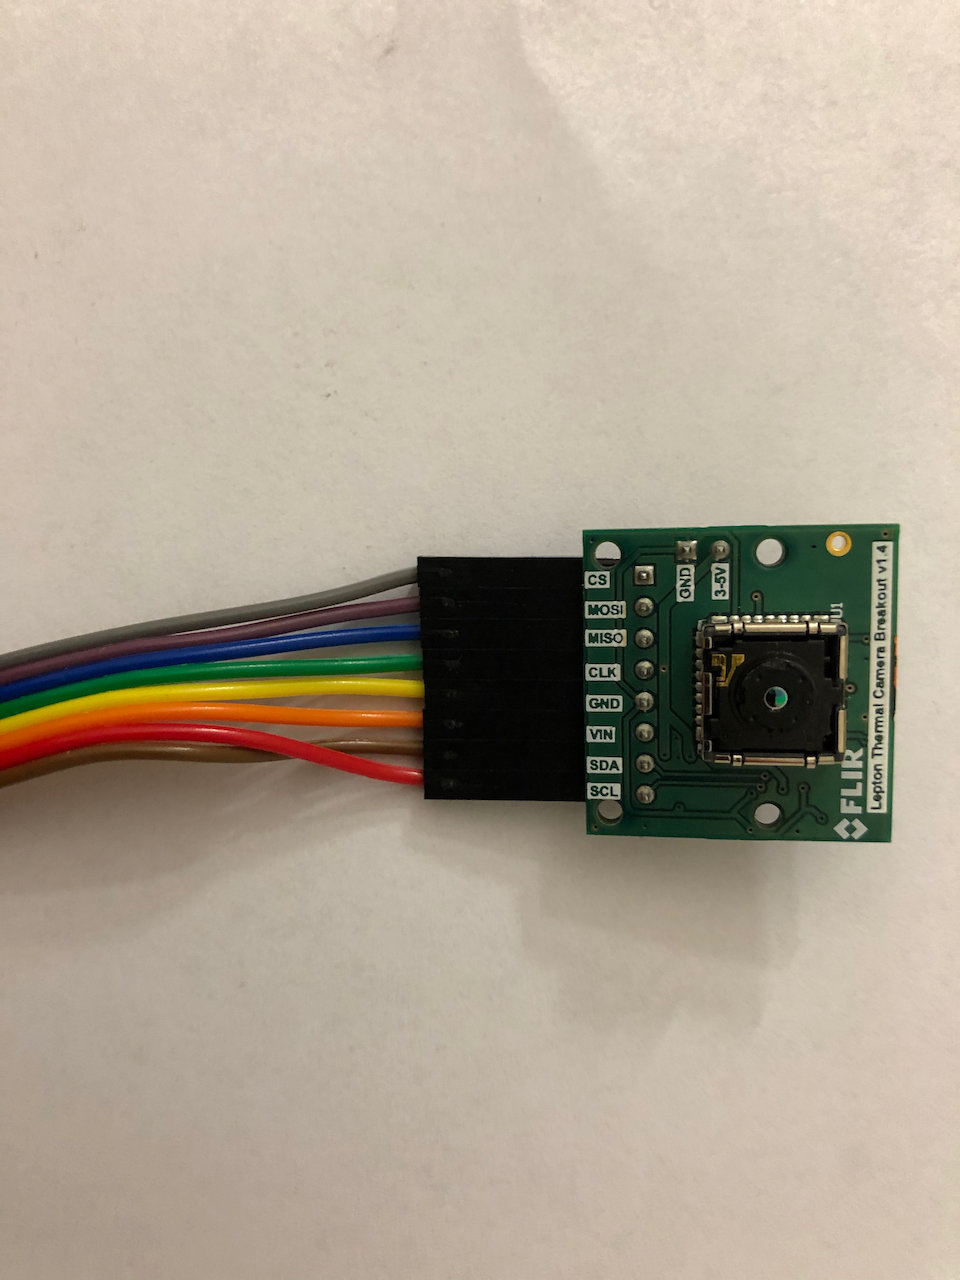
\includegraphics[width=.40\textwidth]{IMG_0361.jpg}} \quad
    \subfloat[][\emph{Top view}.\label{subfig:top.view-gpio}]
        {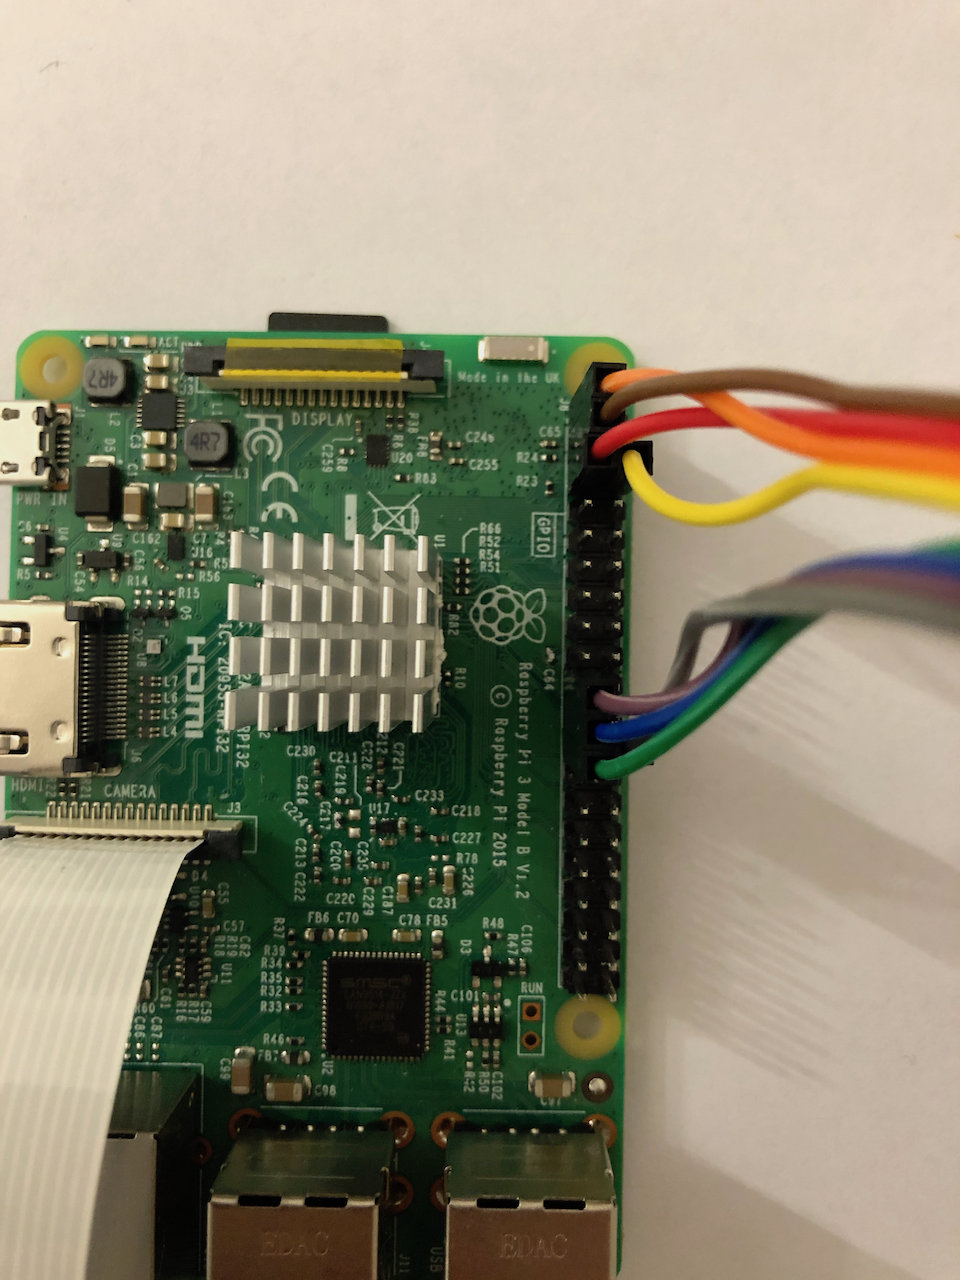
\includegraphics[width=.40\textwidth]{IMG_0362.jpg}} \\
            \subfloat[][\emph{Frontal view}.\label{subfig:front-view-gpio}]
        {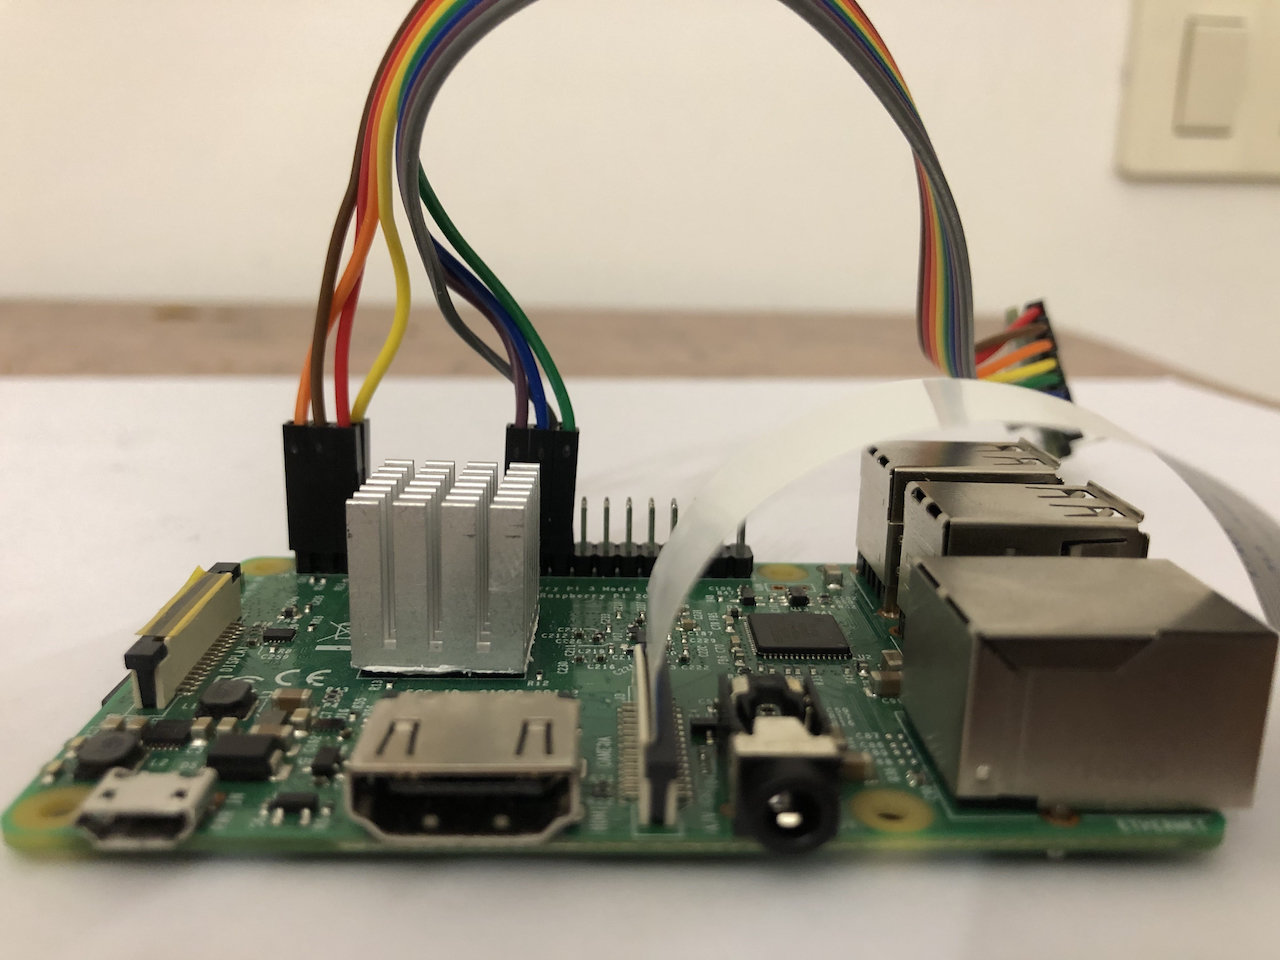
\includegraphics[width=.5\textwidth]{IMG_0360.jpg}}
    \caption{Realization of the connection between the Raspberry Pi 3 GPIO and Break out board}
    \label{fig:brekout-gpio}
\end{figure}

\section{Coral Dev-Board}
\label{sec:hard-devboard}
The Coral Dev Board is a single-board computer that contains an Edge TPU
coprocessor. It's ideal for prototyping new projects that demand fast on-device
inferencing for machine learning models.
%
\begin{figure}[htb]
	\centering
  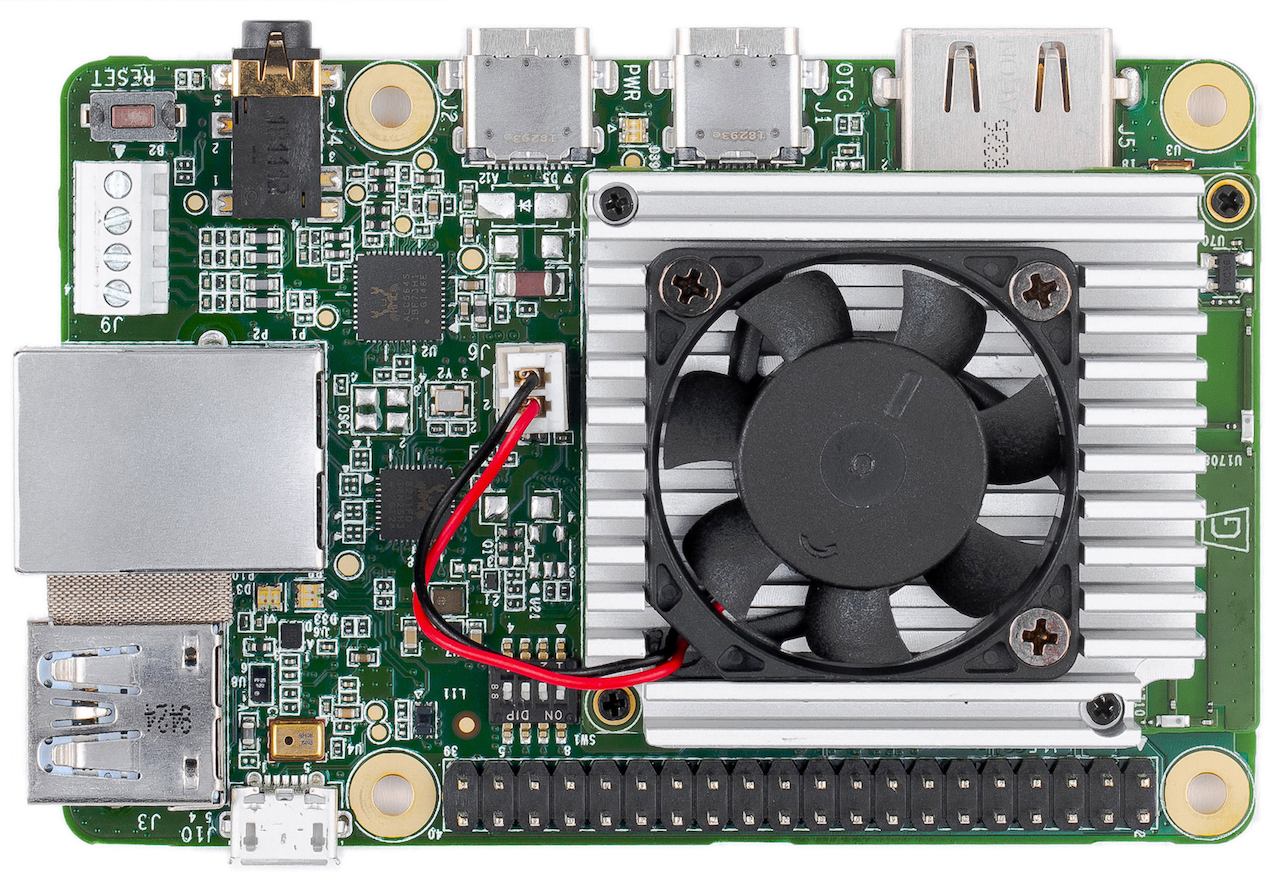
\includegraphics[width=0.80\textwidth]{devboard-dimensions.jpg}
  \captionsource{Coral Dev Board.}{
  \href{https://coral.ai/docs/dev-board/get-started/}{https://coral.ai/docs/dev-board/get-started/}}
  \label{fig:dev-board}
\end{figure}
%
\subsection{Overview}
\label{ssec:hard-devboard-overview}
The Coral Dev Board is a single-board computer that's ideal when you need to
perform fast machine learning (ML) inferencing in a small form factor. You can
use the Dev Board to prototype your embedded system and then scale to production
using the on-board Coral System-on-Module (SoM) combined with your custom PCB
hardware. The SoM provides a fully-integrated system, including NXP's iMX 8M
system-on-chip (SoC), eMMC memory, LPDDR4 RAM, Wi-Fi, and Bluetooth, but its
unique power comes from Google's Edge TPU coprocessor. The Edge TPU is a small
ASIC designed by Google that provides high performance ML inferencing with a low
power cost. For example, it can execute state-of-the-art mobile vision models
such as MobileNet v2 at almost 400 FPS, in a power efficient manner. 
The baseboard provides all the peripheral connections you need to prototype a
project, including USB 2.0/3.0 ports, DSI display interface, CSI-2 camera
interface, Ethernet port, speaker terminals, and a 40-pin I/O header. \hfill \break
Key benefits of the Dev Board:
\begin{itemize}
	\item High-speed and low-power ML inferencing (4 TOPS @ 2 \si{\watt})
	\item A complete Linux system (running Mendel, a Debian derivative)
	\item Prototyping and evaluation board for the small Coral SoM (40 x 48 \si{\milli\meter})
\end{itemize}
%
\begin{table}[htb]
	\centering
	\begin{tabular}{c}
	\hline \\
Edge TPU System-on-Module (SoM)\\
% NXP i.MX 8M SoC (Quad-core Arm Cortex-A53, plus Cortex-M4F)
% Google Edge TPU ML accelerator coprocessor
% Cryptographic coprocessor
% Wi-Fi 2x2 MIMO (802.11b/g/n/ac 2.4/5 GHz)
% Bluetooth 4.2
% 8 GB eMMC
% 1 GB LPDDR4
% USB connections
% USB Type-C power port (5 V DC)
% USB 3.0 Type-C OTG port
% USB 3.0 Type-A host port
% USB 2.0 Micro-B serial console port
% Audio connections
% 3.5 mm audio jack (CTIA compliant)
% Digital PDM microphone (x2)
% 2.54 mm 4-pin terminal for stereo speakers
% Video connections
% HDMI 2.0a (full size)
% 39-pin FFC connector for MIPI DSI display (4-lane)
% 24-pin FFC connector for MIPI CSI-2 camera (4-lane)
% MicroSD card slot
% Gigabit Ethernet port
% 40-pin GPIO expansion header
% Supports Mendel Linux (derivative of Debian)
\hline
	\end{tabular}
	\caption{Coral Dev Board Features.}
	\label{tab:hard-devboard-spec}
\end{table}
%
\noindent The Google Coral with a special TPU chip
performing all tensor calculationsworks with special 
pre-compiled TensorFlow Lite networks. If the topology of the neural network and
its required operations can be described in TensorFlow it may work well on the
Google Coral. However, with its sparse 1 Gbyte RAM, memory shortage can still be
an issue. The Google USB accelerator has its special back-end compiler
converting a TensorFlow Lite file to an executable model for the dongle
TPU.
% 
%
\section{TPU explained in depth}
\label{sec:hard-tpu}
% cite page https://qengineering.eu/google-corals-tpu-explained.html
The Google Coral has a TPU on board which speeds up the tensor calculations
enormously. These tensor calculations are used in deep learning and neural
networks. \hfill \break 
The Google Coral Dev board use an ASIC made by the Google team called the Edge 
TPU. It is a much lighter version of the well-known TPUs used in Google's 
datacenter. \hfill \break
It also consumes very little power, so it is ideal for small embedded systems. 
Nevertheless, the similarities in applied technology are significant.\cite{TPU:explained} 
%
\subsection{Neural Node}
\label{ssec:hard-neural-node}
Neural networks used in deep learning consists of many neural nodes. They are
all connected together in a defined way. The way these nodes are wired is
called the topology of the network. This topology determines the function the
network performs. See this list for a selection of several types of deep
learning networks. Each node has always three basic components. 
A multiplier multiplies all the inputs with their respective so-called weight,
the synapses. An adder who accumulates all the individual multiplications. And
an activation function that shapes the output given the addition. A schematic
view below (\ref{fig:neuron}).\hfill \break
%
\begin{figure}[htb]
	\centering
  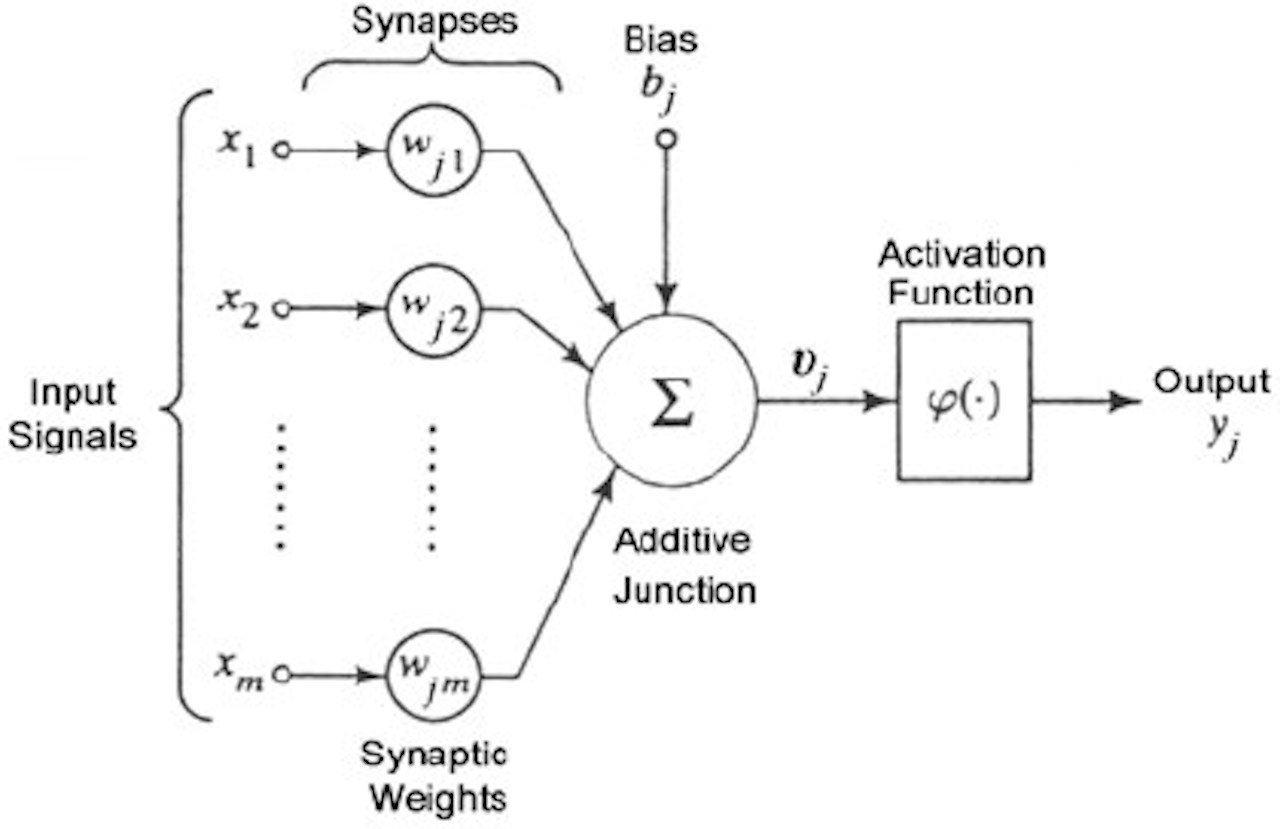
\includegraphics[width=0.70\textwidth]{sinapse.jpg}
  \captionsource{Artificial Neuron models and its parts.}{Adapted from Haykin (1994)}
  \label{fig:neuron}
\end{figure}
%
\newpage
\noindent The formula can be written as follows \eqref{eq:neuron}.
\begin{equation}
\label{eq:neuron}
	y_{i} = \phi \, \left(\sum_{i=1}^{n} w_{ij}\cdot x_{i} \right)
\end{equation}
%
Deep neural network is consist of millions of neural nodes distribute over many
layers; despite the simplicity of the operation, only on multiplication and one
addition, require long compute time to obtain a result. keep in mind that for
training a network requires many epochs. In other words, the main problem is
time. The algorithms is well suited for parallel execution. Although
distributing the algorithm over the processes and threads can be an option
actually provides disappoint results for the presence of bottlenecks due to
architecture general purpose. On the other hand use of Graphical Processing
Unit, the GPU on video card designed for efficient manipulation memory. Their
highly parallel structure make them more efficient respect CPU especially for
algorithms that process large blocks of data in parallel. The best choice is the
use of the Tensor Processing Unit, the TPU. This device has been specially
designed for the above neural node algorithm.
%
\subsection{The adder}
\label{ssec:hard-adder}
Generally a strategy adopted when software is tool slow is modify the hardware
to reach the better achievements.
The structure inside TPU is realized by three main components derived from 
neural node, then keeping in mind the scheme in figure (\ref{fig:neuron}): the 
\textbf{multiplier}, the \textbf{adder} and the \textbf{activation function} 
must be included in the hardware.
Start with analysing the diagram of the 4-bit adder realized in figure
(\ref{fig:4-bit-adder}).
Where: \texttt{A} and \texttt{B} are the inputs. If the output overflows 
\texttt{C4} the carry out is set. \texttt{C0} is the carry-in of a previous 
phase.\cite{TPU:explained}
%
\begin{figure}[!h]
	\centering
  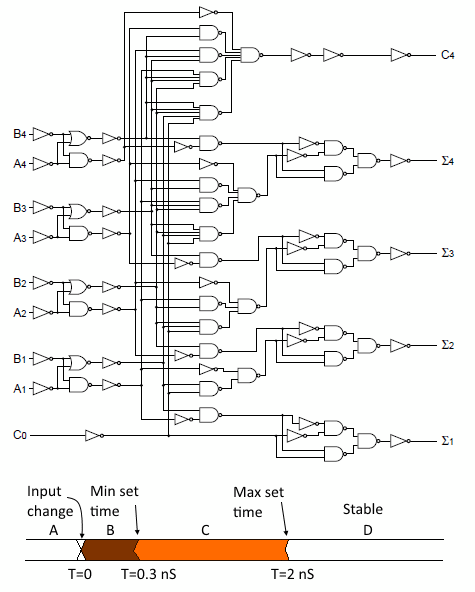
\includegraphics[width=0.75\textwidth]{Adder1.png}
  \captionsource{4-bit adder}{\href{https://qengineering.eu/google-corals-tpu-explained.html}{Q-engineering}}
  \label{fig:4-bit-adder}
\end{figure}
%
Signals \texttt{A} and \texttt{B} propagate through the circuit and generate the
result \texttt{A + B}. Changing one of them alters almost immediately the
output. This happens extremely very fast, within a few nanoseconds. This
propagation time depends on the number of digital ports whose output changes.
The propagation time is therefore not fixed, but lies between two limits, a
minimum and a maximum time, see diagram at the bottom of the drawing
(\ref{fig:4-bit-adder}). By the way, al mentioned times are illustrative and
have no relationship to any device.\cite{TPU:explained}
%
\newpage
\subsection{Pipeline}
\label{ssec:hard-pipeline}
Consider the example where: the propagation time of one adder is $2 \,
\si{\nano\second}$, therefore the maximum clock rate can be $500
\,\si{\mega\hertz}$. Taking into account that a neural node can have many
inputs, also hundreds, that must be accumulated this affect the propagation time
that increase dramatically. This implies that the last adder in the chain must
be attend all intermediate result before its output becomes stable.
If we consider a chain of 250 input each of one with $2\, \si{\nano\second}$
delay, we obtain total time of $500 \,\si{\nano\second}$ waiting. \\
Consequently clock results extremely slow $2\,\si{\mega\hertz}$, then solution
adopted is structured pipeline where between each adder is inserted a memory
element that keep keeps the result stable for the next adder. 
As show in figure (\ref{fig:4-bit-adder-register}). \hfill \break
%
\begin{figure}[!h]
	\centering
	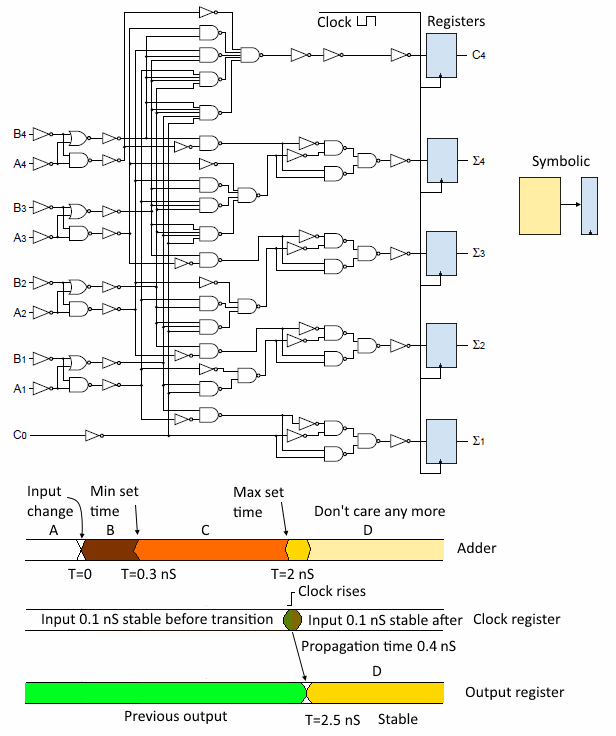
\includegraphics[width=0.75\textwidth]{AdderReg10.png}
	\captionsource{4 bit adder with register}{\href{https://qengineering.eu/google-corals-tpu-explained.html}{Q-engineering}}
	\label{fig:4-bit-adder-register}
\end{figure}
%
\break The output of the registers is updated at the rising edge of the clock
signal. 
That is the only time the output can change. When the clock signal is high or
low, the inputs cannot manipulate the output, then it remains stable. 
Just before the clock rises, the input must be stable for a minimum time, also
just after the rise time. 
In contrast to the previous example, now consider a delay of $0.1
\,\si{\nano\second}$ and adding the register's propagation time of $(0.4
\,\si{\nano\second})$, the total propagation reach for a new stable signal is
now $2.5 \si{\nano\second}$, which results increasing up to clock speed of $400
\,\si{\mega\hertz}$. Observable in figure (\ref{fig:pipe}).
%
\begin{figure}[htb]
	\centering
	\includegraphics[width=0.60\textwidth]{pipe10.png}
	\captionsource{Digital pipeline.}{\href{https://qengineering.eu/google-corals-tpu-explained.html}{Q-engineering}}
	\label{fig:pipe}
\end{figure}
%
%
Taking into account the table in figure \ref{fig:pipe}, each color represents a
value. After four clock cycles, the value at the input has propagated through
the network and appears at the output.
Because the registers are updated simultaneously a new input is accepted every
$2.5 \,\si{\nano\second}$. The propagation time has been restored. 
The time it takes to travel through the whole pipeline is called latency time
and is $10 \,\si{\nano\second}$ in the above diagram $(4 \times 2.5
\,\si{\nano\second}$). 
Every digital component is built on large pipelines which guarantee the required
speed.\cite{TPU:explained}
%
\subsection{The mul-add cell}
\label{ssec:The-mul-add-cell} 
The input signal of every neural node has effect on final result.
This gives a simple multiplication for an input mediate by a weight value. 
The operation of multiplication can be implemented with same logic of an adder,
then are necessary more gates.
Remembering that the neural node has multiplied his value for weight value. 
Thus the representation assume the scheme in figure
(\ref{fig:mul-add-register}). \hfill \break
%
\begin{figure}[htb]
	\centering
	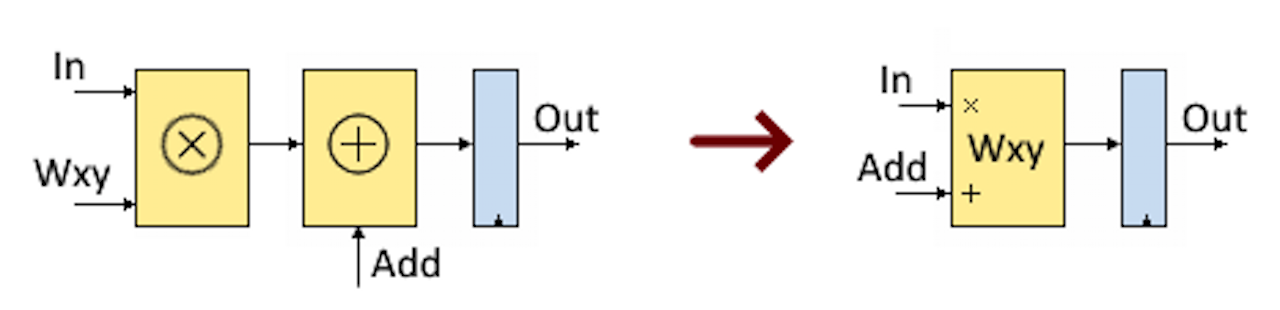
\includegraphics[width=0.65\textwidth]{MulAddReg10.png}
	\captionsource{Mul-Add register.}{\href{https://qengineering.eu/google-corals-tpu-explained.html}{Q-engineering}}
	\label{fig:mul-add-register}
\end{figure}
%
%
%\break For the sake of simplicity, no additional propagation time fixing registers have
%been added. With the formula of the neural node in mind, it is now relatively
%easy to design such a neuron with a few mul-add cells. Below the schematic for a
%three input neuron.
%
\begin{figure}[htb]
	\centering
	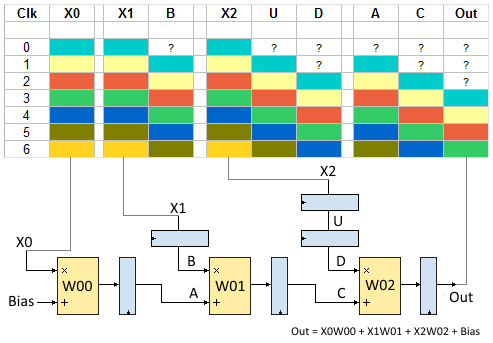
\includegraphics[width=0.75\textwidth]{Neuron.png}
	\captionsource{schematic for a
three input neuron.}{\href{https://qengineering.eu/google-corals-tpu-explained.html}{Q-engineering}}
	\label{fig:3-input-neuron}
\end{figure}
%
%
\newline
Are necessary many important clarifications about the input registers
\texttt{X1} and \texttt{X2} displayed in figure (\ref{fig:3-input-neuron}). They
generate a delay line in the \emph{mul-add} chain, thus can permit to correct
synchronize. Considering the second cell \emph{mul-add} who sum the output from
previous cell (signal \texttt{A}) retarded by one clock cycle. Consequently also
the multiplication between the value in register \texttt{X1} and weight value
must be delayed the same amount of time. The schema reported in figure
(\ref{fig:3-input-neuron}) shows for each colour that represent the vector of
input \texttt{$[X0, X1, X2]$} while the input \texttt{A} and \texttt{B},
represented by lines straight, maintains always same colour. This means that
they appear simultaneous, i.e. are synchronised. The same must be valid for
input \texttt{C} and \texttt{D}.
%
\subsection{Systolic array}
\label{ssec:hard-systolic-array}
Starting from structure, just examined, is quite easy extend it to other neurons, taking into account that every single input is connected with all neurons in the next layer, as shows in figure (\ref{fig:systolic-array-edge-tpu}).
%
\begin{figure}[htb]
	\centering
	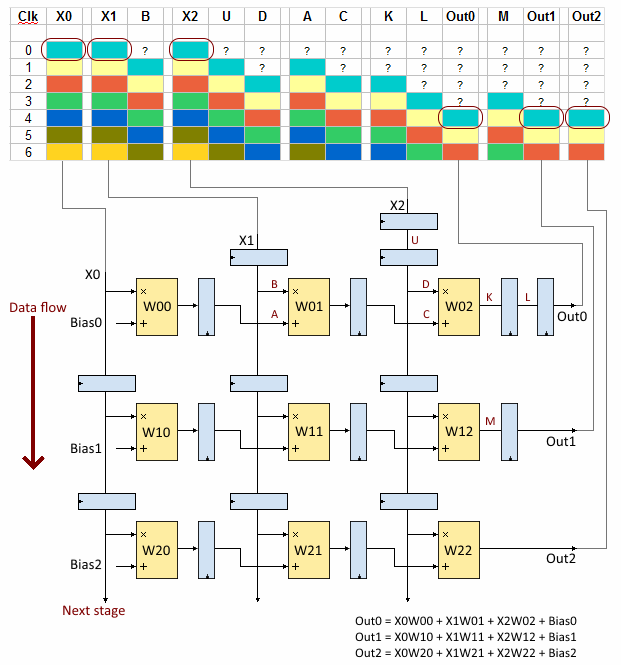
\includegraphics[width=0.65\textwidth]{Systolic-Array.png}
	\captionsource{Systolic Array Edge TPU.}{\href{https://qengineering.eu/google-corals-tpu-explained.html}{Q-engineering}}
	\label{fig:systolic-array-edge-tpu}
\end{figure}
%
%
The adoption of this solution, called systolic array, permits to have an
increment of speed in parallel calculation. 
Since the propagation time remains unchanged for an spread of systolic array in
depth or width, while only the latency time grows up this represent the solution
widely used for neural network hardware.
%
%The sizes of the systolic array in the Edge TPU are not known yet. The first TPU
%Google uses in its datacenter contains 256 x 256 \emph{mul-add} cells. Running at 700
%MHz it can theoretical performs 256 x 256 x 700.000.000 = 46 trillion \emph{mul-adds}
%per second. Or if you look to individual operations 92 trillion (92 TOPS).
%However, this impressive figure is purely theoretical. In practice, there are
%some factors that slow performance.
%
%The systolic array is made up of hardware. This means that it has fixed
%dimensions. Therefore, the input and output vectors also have fixed dimensions.
%However, the numbers of neurons per layer are determined by the design and are
%certainly not constant. If the number is smaller than the size of the array, it
%is, of course, possible to expand an input vector with leading zeros, so that
%the dimension equals the array size. The same technique can be applied to an
%oversized output vector.
%
%If the input vector contains more elements than the width of the systolic array,
%the entire arithmetic calculation must be performed in more than one call. To
%this end, the input vector is cut into a series of smaller vectors that match
%the width of the series. They are then processed one after the other. The
%intermediate results must be stored in a buffer. These values must be added
%after completion of all the systolic calls. Note that not only the input vector
%is split into smaller parts, but all weights used in the multiplication must be
%updated according to the formula's processing section. This may require a
%massive memory transfer. Below an example of a systolic array with only four
%inputs processing a vector of size 12.
%
%
%
%Looking at Google's schematic overview of the TPU, these output buffers and
%accumulators are drawn at the bottom. (In their diagram, the output is at the
%bottom instead of the right as on our drawing).
%Google TPU detail
%
% 
%Buffers have also been placed on the input vector side in the diagram above.
%They act as a first-in-first-out buffer, a FIFO. This guarantees continuous
%input of the systolic array with input values. It may also have some rotating
%operations, which increases the performance of CNN networks. It is unclear
%whether Google uses this method here. 
%
\subsection{Activation unit}
\label{ssec:activation-unit}
Once the output is available, it is sent to the activation unit. This module
within the Edge TPU applies the activation function to the output. It is
hardwired. In other words, you cannot alter the function, it works like a ROM.
Probably it is a ReLU function as it is nowadays the most used activation
function and it is very easy to implement in hardware.\cite{TPU:explained}
%
% 
% TPU versus Edge TPU. The Google's Edge TPU is a much smaller device than the
% TPUs that Google uses in its data centers. Below the PCB with the original TPU
% and the Edge TPU on the same scale. TPU vs Edge TPU It is obvious that such a
% small device cannot have the same functions as its much larger ancestor. The
% floor plan on the die does not allow this to happen. Nor can the systolic
% array have the $256 \times 256$ dimension as in the original TPU. Google has
% so far not revealed the measures in the Edge, but a well-founded estimate is
% $64 \times 64$ with a clock of $480 \si{\mega\hertz}$, resulting in 4 TOPS.
% Memory is also an issue. In the original chip, it takes around $29\%$ of the
% total floor plan. It is impossible that the same amount can be found on the
% Edge TPU die. Moreover, the chip is very energy efficient. It requires no
% cooling. This means that almost certainly all the buffering is outside the
% chip. It leaves only a simple transfer of input vectors, output vectors and
% weights to the chip.  Practice. In fact, that is the whole concept of the
% Google Coral Dev board. Transfer all tensor calculations to the TPU as quickly
% as possible, fetch for the results, fill them in the next layer and start the
% cycle again with this layer. Process all layers one by one until they are
% ready. To speed up the process, TensorFlow uses a special back end compiler,
% the Edge TPU compiler. The main task of this Edge TPU compiler is to partition
% the TensorFlow Lite file into more suitable TPU transfer packages. If for any
% reason the TPU cannot process the TensorFlow Lite file or part of it, the CPU
% will take care of it. However, if this happens, your application will, of
% course, work extremely slowly. 8 bits integers. Another way of speeding up the
% calculations is the use of 8 bit signed integers instead of floats. A floating
% number occupies 32 bits in memory whereas the integer only needs 8. Because a
% neural network is fairly insensitive to number accuracy, it will also work
% well with 8-bit integers. It will still remain accurate. Not only does this
% technology save approximately $75\%$ memory, but it also significantly reduces
% the number of transistors on the chip. If you look at the adder at the top of
% the page, you can imagine how many transistors a floating-point adder needs.
% Without this compression, the Edge TPU would not be as powerful, small and
% energy efficient.

% The converting algorithm from floating point to 8 bit signed integer is quite
% simple. First, it determines which maximum and minimum a variable will take in
% the model. The larger of the two is then taken and scaled to 127. Suppose
% minimum is -1205.8 and maximum is 646.8. The larger is the min value of
% 1205.8. So that number becomes -127. Zero remains zero. That gives 646.8 a
% integer value of 127 x (646.8 / 1205.8) = 68. Every number in the TensorFlow
% model is converted in this way. Not only for the Edge TPU, by the way. All
% TensorFlow Lite models for embedded deep learning are processed in this way.

% A rather remarkable detail is the output of the Edge TPU, which does consist
% of a floating point. Because the activation function is embedded in a ROM, it
% is just as easy to store floating numbers as integers. One last tip in this
% regard. Apply quantization-aware training in TensorFlow. This simulates the
% effect of the 8 bit signed integers. Therefore generating a more precise
% model. It makes the model also more tolerant for low precision variables.
\section{TPU explained in depth}
\label{sec:hard-tpu}
% cite page https://qengineering.eu/google-corals-tpu-explained.html
The Google Coral has a TPU on board which speeds up the tensor calculations
enormously. These tensor calculations are used in deep learning and neural
networks. \hfill \break 
The Google Coral Dev board use an ASIC made by the Google team called the Edge 
TPU. It is a much lighter version of the well-known TPUs used in Google's 
datacenter. \hfill \break
It also consumes very little power, so it is ideal for small embedded systems. 
Nevertheless, the similarities in applied technology are significant.\cite{TPU:explained} 
%
\subsection{Neural Node}
\label{ssec:hard-neural-node}
Neural networks used in deep learning consists of many neural nodes. They are
all connected together in a defined way. The way these nodes are wired is
called the topology of the network. This topology determines the function the
network performs. See this list for a selection of several types of deep
learning networks. Each node has always three basic components. 
A multiplier multiplies all the inputs with their respective so-called weight,
the synapses. An adder who accumulates all the individual multiplications. 
And an activation function that shapes the output given the addition. A
schematic view below (\ref{fig:neuron}).\hfill \break
%
\begin{figure}[htb]
	\centering
	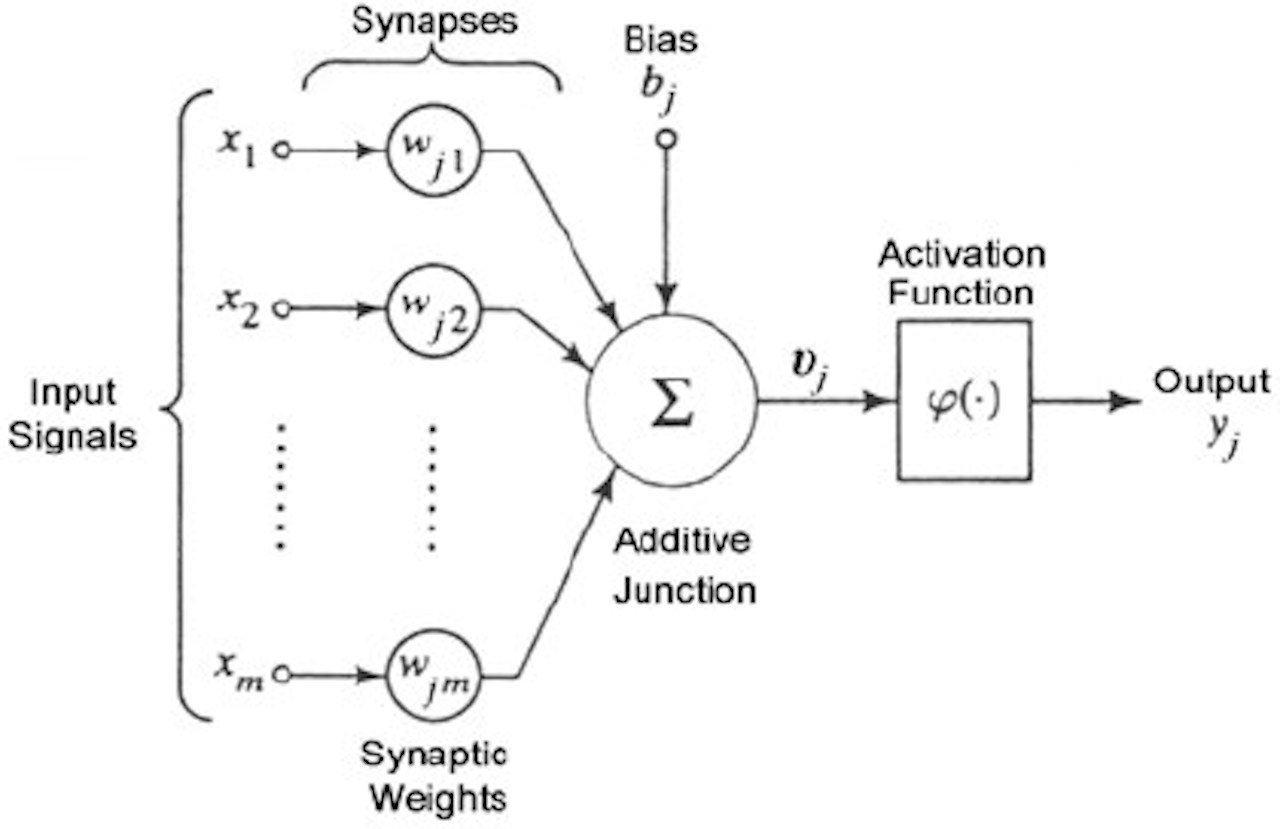
\includegraphics[width=0.70\textwidth]{sinapse.jpg}
	\captionsource{Artificial Neuron models and its parts.}{Adapted from Haykin (1994)}
	\label{fig:neuron}
\end{figure}
%
\newpage
\noindent The formula can be written as follows \eqref{eq:neuron}.
\begin{equation}
\label{eq:neuron}
	y_{i} = \phi \, \left(\sum_{i=1}^{n} w_{ij}\cdot x_{i} \right)
\end{equation}
%
Deep neural network is consist of millions of neural nodes distribute over many
layers; despite the simplicity of the operation, only on multiplication and one
addition, require long compute time to obtain a result. keep in mind that for
training a network requires many epochs. In other words, the main problem is
time. The algorithms is well suited for parallel execution. Although
distributing the algorithm over the processes and threads can be an option
actually provides disappoint results for the presence of bottlenecks due to
architecture general purpose. On the other hand use of Graphical Processing
Unit, the GPU on video card designed for efficient manipulation memory. Their
highly parallel structure make them more efficient respect CPU especially for
algorithms that process large blocks of data in parallel. The best choice is the
use of the Tensor Processing Unit, the TPU. This device has been specially
designed for the above neural node algorithm.
%
\subsection{The adder}
\label{ssec:hard-adder}
Generally a strategy adopted when software is tool slow is modify the hardware
to reach the better achievements.
The structure inside TPU is realized by three main components derived from 
neural node, then keeping in mind the scheme in figure (\ref{fig:neuron}): the 
\textbf{multiplier}, the \textbf{adder} and the \textbf{activation function} 
must be included in the hardware.
Start with analysing the diagram of the 4-bit adder realized in figure
(\ref{fig:4-bit-adder}).\hfill \break
Where: \texttt{A} and \texttt{B} are the inputs. If the output overflows 
\texttt{C4} the carry out is set. \texttt{C0} is the carry-in of a previous 
phase.\cite{TPU:explained}
%
\begin{figure}[!h]
	\centering
	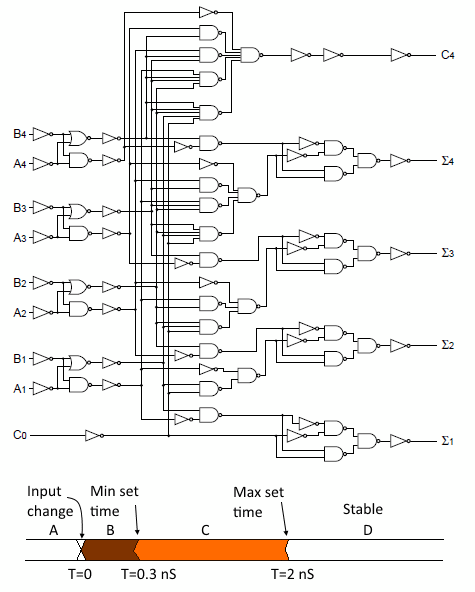
\includegraphics[width=0.75\textwidth]{Adder1.png}
	\captionsource{4-bit adder}{\href{https://qengineering.eu/google-corals-tpu-explained.html}{Q-engineering}}
	\label{fig:4-bit-adder}
\end{figure}
%
Signals \texttt{A} and \texttt{B} propagate through the circuit and generate the
result \texttt{A + B}. Changing one of them alters almost immediately the
output. This happens extremely very fast, within a few nanoseconds. This
propagation time depends on the number of digital ports whose output changes.
The propagation time is therefore not fixed, but lies between two limits, a
minimum and a maximum time, see diagram at the bottom of the drawing
(\ref{fig:4-bit-adder}). By the way, al mentioned times are illustrative and
have no relationship to any device.\cite{TPU:explained}
%
\newpage
\subsection{Pipeline}
\label{ssec:hard-pipeline}
Consider the example where: the propagation time of one adder is $2 \,
\si{\nano\second}$, therefore the maximum clock rate can be $500
\,\si{\mega\hertz}$. Taking into account that a neural node can have many
inputs, also hundreds, that must be accumulated this affect the propagation time
that increase dramatically. This implies that the last adder in the chain must
be attend all intermediate result before its output becomes stable. 
If we consider a chain of 250 input each of one with $2\, \si{\nano\second}$
delay, we obtain total time of $500 \,\si{\nano\second}$ waiting. \\ 
Consequently clock results extremely slow $2\,\si{\mega\hertz}$, then solution
adopted is structured pipeline where between each adder is inserted a memory
element that keep keeps the result stable for the next adder. 
As show in figure (\ref{fig:4-bit-adder-register}). \hfill \break
%
\begin{figure}[!h]
	\centering
	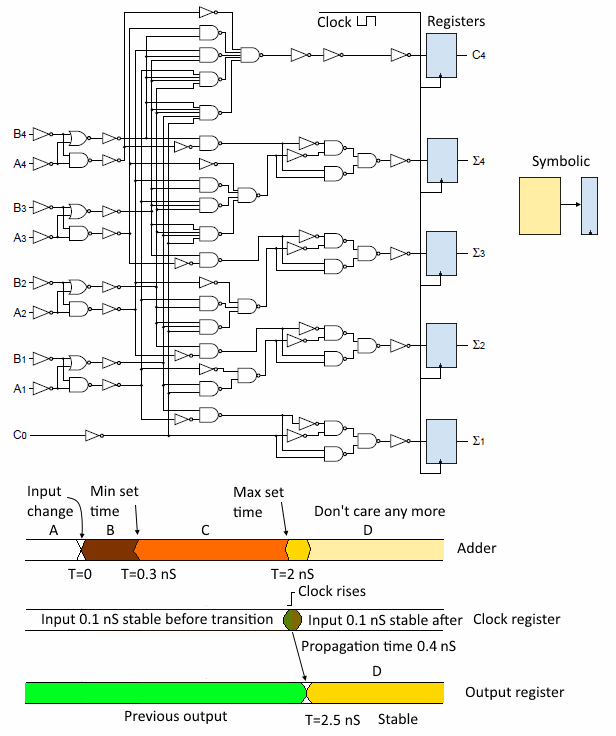
\includegraphics[width=0.75\textwidth]{AdderReg10.png}
	\captionsource{4 bit adder with register}{\href{https://qengineering.eu/google-corals-tpu-explained.html}{Q-engineering}}
	\label{fig:4-bit-adder-register}
\end{figure}
%
\break The output of the registers is updated at the rising edge of the clock
signal. That is the only time the output can change. When the clock signal is
high or low, the inputs cannot manipulate the output, then it remains stable. 
Just before the clock rises, the input must be stable for a minimum time, also
just after the rise time. In contrast to the previous example, now consider a
delay of $0.1 \,\si{\nano\second}$ and adding the register's propagation time of
$(0.4 \,\si{\nano\second})$, the total propagation reach for a new stable signal
is now $2.5 \,\si{\nano\second}$, which results increasing up to clock speed of
$400 \,\si{\mega\hertz}$. Observable in figure (\ref{fig:pipe}). \hfill \break
%
\begin{figure}[htb]
	\centering
	\includegraphics[width=0.60\textwidth]{pipe10.png}
	\captionsource{Digital pipeline.}{\href{https://qengineering.eu/google-corals-tpu-explained.html}{Q-engineering}}
	\label{fig:pipe}
\end{figure}
%
%
\newline
Taking into account the table in figure (\ref{fig:pipe}), each color represents a
value. After four clock cycles, the value at the input has propagated through
the network and appears at the output.	Because the registers are updated
simultaneously a new input is accepted every $2.5 \,\si{\nano\second}$.	The
propagation time has been restored. The time it takes to travel through the
whole pipeline is called latency time and is $10 \,\si{\nano\second}$ in the
above diagram $(4 \times 2.5 \,\si{\nano\second}$). Every digital component is
built on large pipelines which guarantee the required speed.\cite{TPU:explained}
 
%
\subsection{The mul-add cell}
\label{ssec:The-mul-add-cell} 
The input signal of every neural node has effect on final result. This gives a
simple multiplication for an input mediate by a weight value. The operation of
multiplication can be implemented with same logic of an adder, then are
necessary more gates. 
Remembering that the neural node has multiplied his value for weight value. 
Thus the representation assume the scheme in figure
(\ref{fig:mul-add-register}).
%
\begin{figure}[htb]
	\centering
	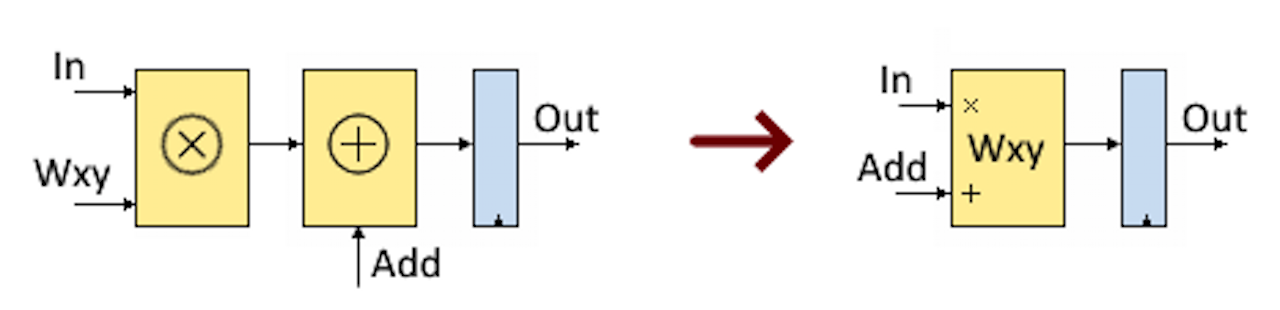
\includegraphics[width=0.65\textwidth]{MulAddReg10.png}
	\captionsource{Mul-Add register.}{\href{https://qengineering.eu/google-corals-tpu-explained.html}{Q-engineering}}
	\label{fig:mul-add-register}
\end{figure}
%
%
%\break For the sake of simplicity, no additional propagation time fixing registers have
%been added. With the formula of the neural node in mind, it is now relatively
%easy to design such a neuron with a few mul-add cells. Below the schematic for a
%three input neuron.
%
\begin{figure}[htb]
	\centering
	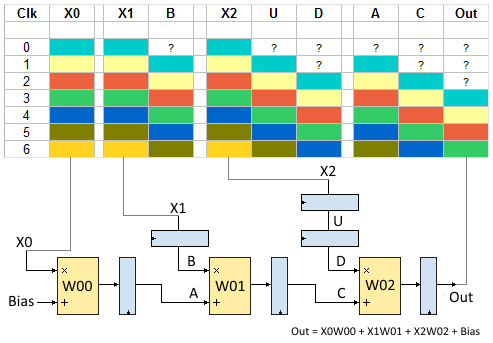
\includegraphics[width=0.75\textwidth]{Neuron.png}
	\captionsource{Schematic for a
three input neuron.}{\href{https://qengineering.eu/google-corals-tpu-explained.html}{Q-engineering}}
	\label{fig:3-input-neuron}
\end{figure}
%
%
Are necessary many important clarifications about the input registers
\texttt{X1} and \texttt{X2} displayed in figure (\ref{fig:3-input-neuron}). They
generate a delay line in the \emph{mul-add} chain, thus can permit to correct
synchronize. Considering the second cell \emph{mul-add} who sum the output from
previous cell (signal \texttt{A}) retarded by one clock cycle. Consequently also
the multiplication between the value in register \texttt{X1} and weight value
must be delayed the same amount of time. The schema reported in figure
(\ref{fig:3-input-neuron}) shows for each colour that represent the vector of
input \texttt{$[X0, X1, X2]$} while the input \texttt{A} and \texttt{B},
represented by lines straight, maintains always same colour. This means that
they appear simultaneous, i.e. are synchronised. The same must be valid for
input \texttt{C} and \texttt{D}.
%
\subsection{Systolic array}
\label{ssec:hard-systolic-array}
Starting from structure, just examined, is quite easy extend it to other
neurons, taking into account that every single input is connected with all
neurons in the next layer, as shows in figure
(\ref{fig:systolic-array-edge-tpu}).
%
\begin{figure}[htb]
	\centering
	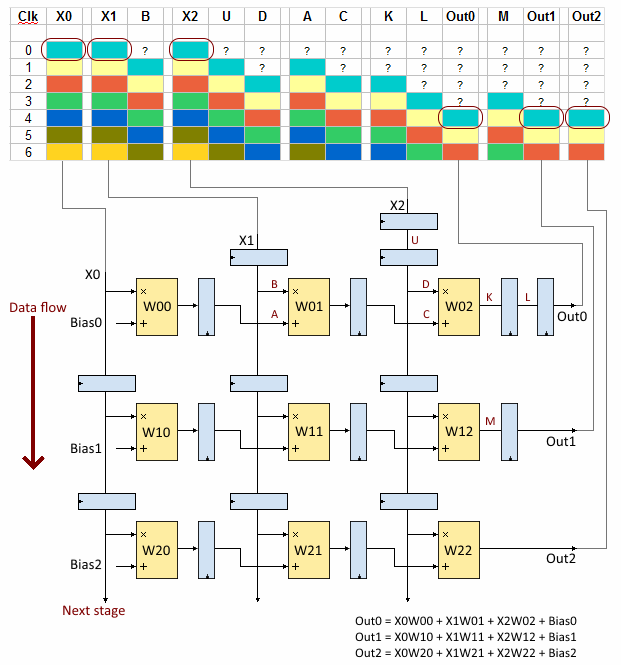
\includegraphics[width=0.75\textwidth]{Systolic-Array.png}
	\captionsource{Systolic Array Edge TPU.}{\href{https://qengineering.eu/google-corals-tpu-explained.html}{Q-engineering}}
	\label{fig:systolic-array-edge-tpu}
\end{figure}
%
%
The adoption of this solution, called systolic array, permits to have an
increment of speed in parallel calculation. 
Since the propagation time remains unchanged for an spread of systolic array in
depth or width, while only the latency time grows up this represent the solution
widely used for neural network hardware.
%
%The sizes of the systolic array in the Edge TPU are not known yet. The first TPU
%Google uses in its datacenter contains 256 x 256 \emph{mul-add} cells. Running at 700
%MHz it can theoretical performs 256 x 256 x 700.000.000 = 46 trillion \emph{mul-adds}
%per second. Or if you look to individual operations 92 trillion (92 TOPS).
%However, this impressive figure is purely theoretical. In practice, there are
%some factors that slow performance.
%
%The systolic array is made up of hardware. This means that it has fixed
%dimensions. Therefore, the input and output vectors also have fixed dimensions.
%However, the numbers of neurons per layer are determined by the design and are
%certainly not constant. If the number is smaller than the size of the array, it
%is, of course, possible to expand an input vector with leading zeros, so that
%the dimension equals the array size. The same technique can be applied to an
%oversized output vector.
%
%If the input vector contains more elements than the width of the systolic array,
%the entire arithmetic calculation must be performed in more than one call. To
%this end, the input vector is cut into a series of smaller vectors that match
%the width of the series. They are then processed one after the other. The
%intermediate results must be stored in a buffer. These values must be added
%after completion of all the systolic calls. Note that not only the input vector
%is split into smaller parts, but all weights used in the multiplication must be
%updated according to the formula's processing section. This may require a
%massive memory transfer. Below an example of a systolic array with only four
%inputs processing a vector of size 12.
%
%
%
%Looking at Google's schematic overview of the TPU, these output buffers and
%accumulators are drawn at the bottom. (In their diagram, the output is at the
%bottom instead of the right as on our drawing).
%Google TPU detail
%
% 
%Buffers have also been placed on the input vector side in the diagram above.
%They act as a first-in-first-out buffer, a FIFO. This guarantees continuous
%input of the systolic array with input values. It may also have some rotating
%operations, which increases the performance of CNN networks. It is unclear
%whether Google uses this method here. 
%
%
\subsection{Activation unit}
\label{ssec:activation-unit}
Once the output is available, it is sent to the activation unit. This module
within the Edge TPU applies the activation function to the output. It is
hardwired. In other words, you cannot alter the function, it works like a ROM.
Probably it is a ReLU function as it is nowadays the most used activation
function and it is very easy to implement in hardware.\cite{TPU:explained}
%
%
% TPU versus Edge TPU. The Google's Edge TPU is a much smaller device than the
% TPUs that Google uses in its data centers. Below the PCB with the original TPU
% and the Edge TPU on the same scale. TPU vs Edge TPU It is obvious that such a
% small device cannot have the same functions as its much larger ancestor. The
% floor plan on the die does not allow this to happen. Nor can the systolic
% array have the $256 \times 256$ dimension as in the original TPU. Google has
% so far not revealed the measures in the Edge, but a well-founded estimate is
% $64 \times 64$ with a clock of $480 \si{\mega\hertz}$, resulting in 4 TOPS.
% Memory is also an issue. In the original chip, it takes around $29\%$ of the
% total floor plan. It is impossible that the same amount can be found on the
% Edge TPU die. Moreover, the chip is very energy efficient. It requires no
% cooling. This means that almost certainly all the buffering is outside the
% chip. It leaves only a simple transfer of input vectors, output vectors and
% weights to the chip.	
% Practice.
